\documentclass{article}
\usepackage[utf8]{inputenc}
\usepackage[english]{babel}
\usepackage{indentfirst}
\usepackage{graphicx}
\usepackage{xcolor}
\usepackage{amsmath}
\usepackage{hyperref}

\newcommand{\cmd}[1]{\texttt{#1}}
\newcommand{\ib}[1]{\textbf{\textit{#1}}}
\hypersetup{
	colorlinks = true,
	linkbordercolor = 1 1 1,
	urlcolor = blue,
	linkcolor = black,
	urlbordercolor = 1 1 1,
	citecolor = black
}


\title{Serious Game\\Rapport de la 3ème étape}
\author{}
\date{}
\addto\captionsenglish{\renewcommand*\contentsname{Sommaire}}


\pagestyle{headings}

\begin{document}

\begin{titlepage}
	\begin{center}

		% \vspace* creates some vertical white space on the page to make the title page look more pleasing.  \vspace would do much the same thing, but would not insert the white space if we were at the top of a fresh page.  As this is the start of the document we're obviously at the beginning of a page, so the asterisk is necessary to ensure we still put in two cm of white space.
		\vspace*{2cm}
		
		{\Large Services et technologies multimédia (D200006)} % \huge sets the font size.  Other options include things like \large, \Large, \small, \tiny, etc.
		
		\vspace{5cm}
		{\huge\textbf{Projet Unity, Serious Game\\Rapport de la 3ème étape:\\ }}
		
		\vspace{4cm}
		{par\\\large Dany A. DARGHOUTH \\\& Cédric PENDVILLE}
		% \vfill creates an arbitrary amount of vertical white space as necessary to fill the page
		\vfill
		
		Juin 2023
		
		% \vspace*{3cm}
		
		\end{center}
\end{titlepage}

\maketitle
\tableofcontents
\newpage

\section{Introduction}
Ce rapport accompagne le rendu de la 3ème étape du projet de serious games dans le cadre du cours de Services et technologies multimédia.\\

Le jeu développé s'appelle Tilogic est est un jeu de réflexion basé sur la logique booléenne. Le joueur doit résoudre des niveaux en utilisant des portes logiques. Le projet s'adresse à un public (jeune ou moins jeune) qui n'a ni expérience dans les jeux vidéo ni connaissance de la logique booléenne et se veut une introduction ludique à ce dernier domaine.\\

\section{Gameplay}
Étant une introduction à un domaine complexe, le jeu en lui-même ne pouvait pas proposer un gameplay trop compliqué et rester abordable pour un public non averti, le style puzzle/point and click s'est donc montré le plus pertinent.\\

\section{Règles du jeu}
Les règles du jeu sont simples, un niveau prend la forme d'un circuit logique à trous que le joueur doit compléter en utilisant les portes logiques mises à sa disposition de sorte à ce que toutes les lampes "output" soient allumées.\\

Le score du joeur est calculé de la manière suivante: Chaque ensemble de niveau
réussi (complété dans le temps imparti) rapporte 1 étoile, le meilleur score possible étant 5 étoiles.\\


\section{But du jeu}
Le but du jeu est de résoudre les niveaux proposés en utilisant les portes logiques mises à disposition, le plus vite possible afin d'obtenir le meilleur score.\\

D'un point de vu plus général, le but du jeu est d'apprendre les bases de la logique booléenne de manière ludique et d'introduire ce domaine à un publique qui n'est pas forcémment familier avec les jeux vidéos ou la logique.\\

\section{Adapatation de la difficulté}
L'adapatation de la difficulté s'eefectue de la manière suivante: Le temps que le joueur met à résoudre un niveau est mesuré, et si le temps mis est en dessous d'un certain seuil, le joueur se vera proposé un niveau présentatn une nouvelle porte logique, dans le cas contraire, le jeu lui proposera un nouveau niveau n'incluant que la/les portes qu'il connait déjà. Cette différence influear également sur le score du joueur (le meilleur score étant obtenu en résolvant tous les niveaux "assez" rapidement).\\

\begin{figure}[h]
    \centering
    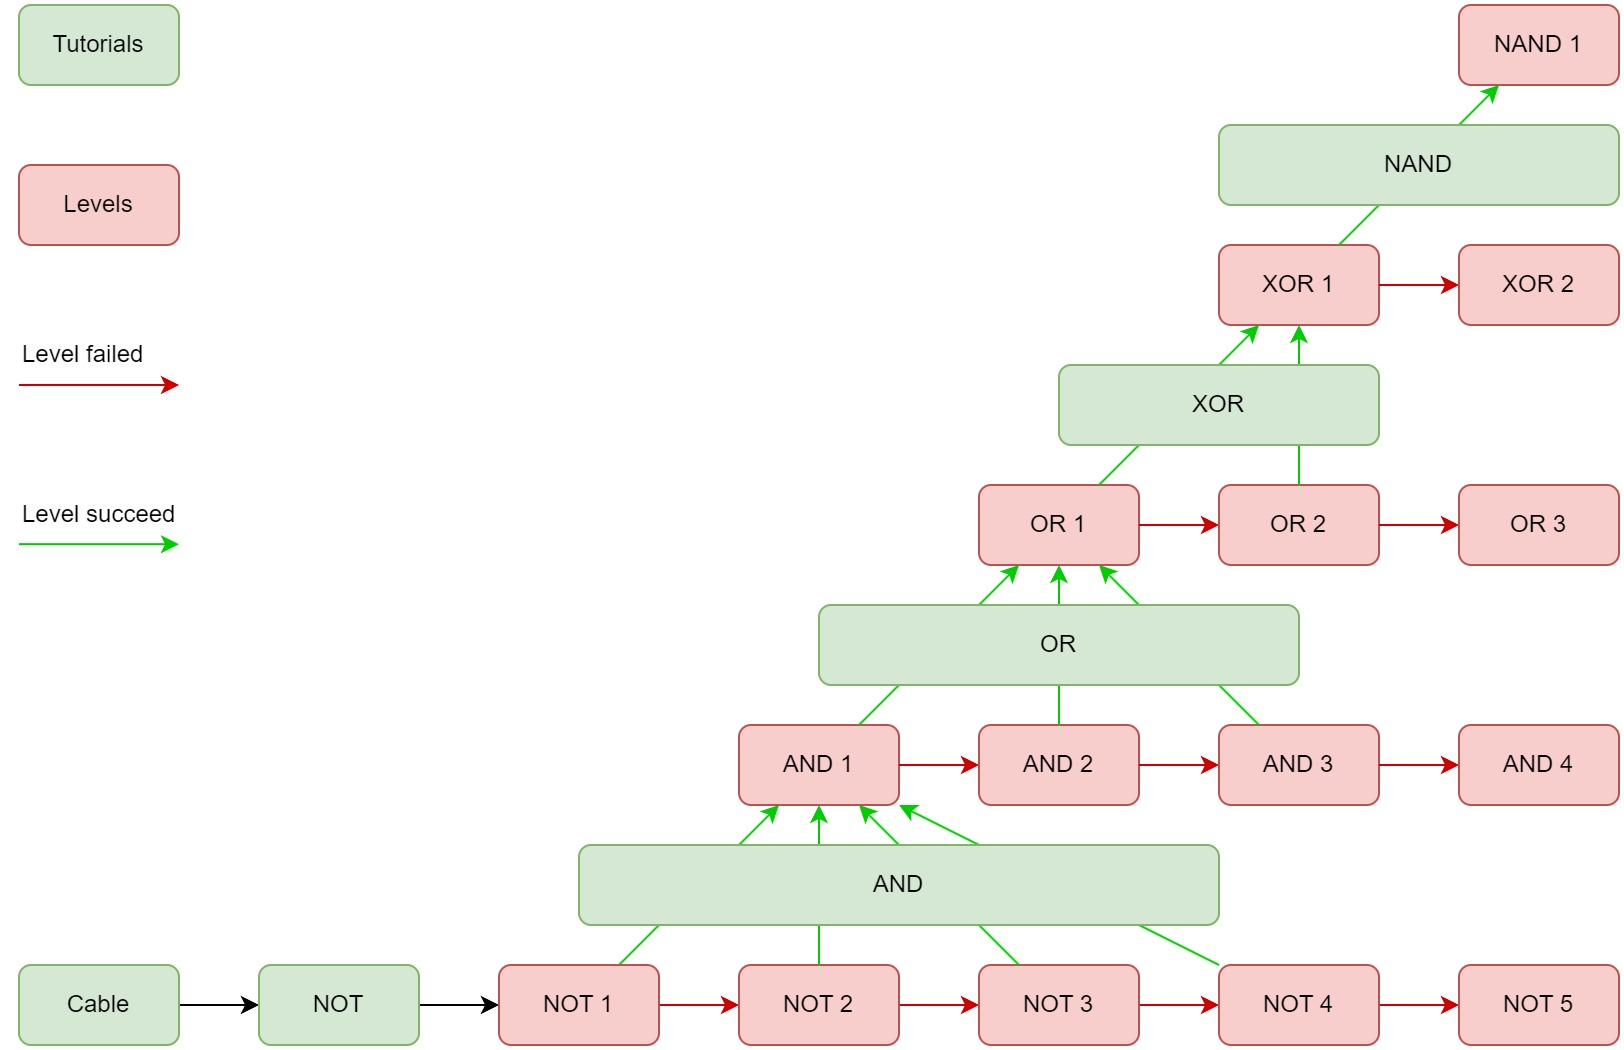
\includegraphics[width=\textwidth]{img/Levels Tree.jpg}
    \caption{Schéma de la structure des niveaux}
\end{figure}

\section{Structure du jeu}
    \subsection{Scènes}

    Chaque scène de jeu est composée d'un board, de portes logiques et d'un script qui modifie l'état des cables en implémentant une vraie logique.

    \subsection{GameObjects}
    \noindent
    Les GameObjects les plus importants sont les suivants
    \begin{enumerate}
        \item \ib{Gates} : les portes logiques, divisées en 2 catégories, 2 points et 3 points.
        \item \ib{Emitter} : les lumière de gauche, fixes.
        \item \ib{Goal} : les lumière de droite, qui s'adapte à l'état des cables.
        \item \ib{Snapping point} : les endroits où les portes logiques peuvent se "fixer".
    \end{enumerate}
    
    \subsection{Scripts}
    \noindent
    Les scripts les plus importants sont les suivants
    \begin{enumerate}
        \item \ib{Scripts de niveau} : allume les cables en fonction des portes placées et valide le niveau s'il est réussi.
        \item \ib{Draggable} : permet de déplacer les portes (et tout autre objet ayant un Box collider) et de les fixer sur les snapping points.
        \item \ib{Chrono} : affiche le chronomètre et déclare un échec du niveau si le temps est écoulé.
        \item \ib{Extract\_time} : script de debug permettant d'extraire le temps que mettent les utilisateurs à finir chaque niveau.
    \end{enumerate}

\section{Evaluation du jeu}
\textit{L'évaluation du jeu n'a pas été faite par un autre groupe, mais plutôt par des proches et certains camarades. Les tests ont été fait sur la version précédant la version finale, donc les points faibles ont été corrigés.}
	\subsection{Points forts}
    \begin{itemize}
        \item Concept.
        \item Simplicité de lecture.
        \item Aspect ludique.
    \end{itemize}
	\subsection{Points faibles}
    \begin{itemize}
        \item Manque de clarté au niveau des portes logiques (manque de séparation des 2 types de portes).
        \item Manque de clarté du but du jeu.
    \end{itemize}
	\subsection{Améliorations possibles}
    \begin{itemize}
        \item Plus de niveaux.
        \item Des niveaux plus durs.
        \item Des niveaux plus simples.
        \item De la musique en jeu.
        \item Un système de Leaderboard.
    \end{itemize}

\newpage
\section{Annexe : Les niveaux}
\begin{figure}[h]
    \centering
    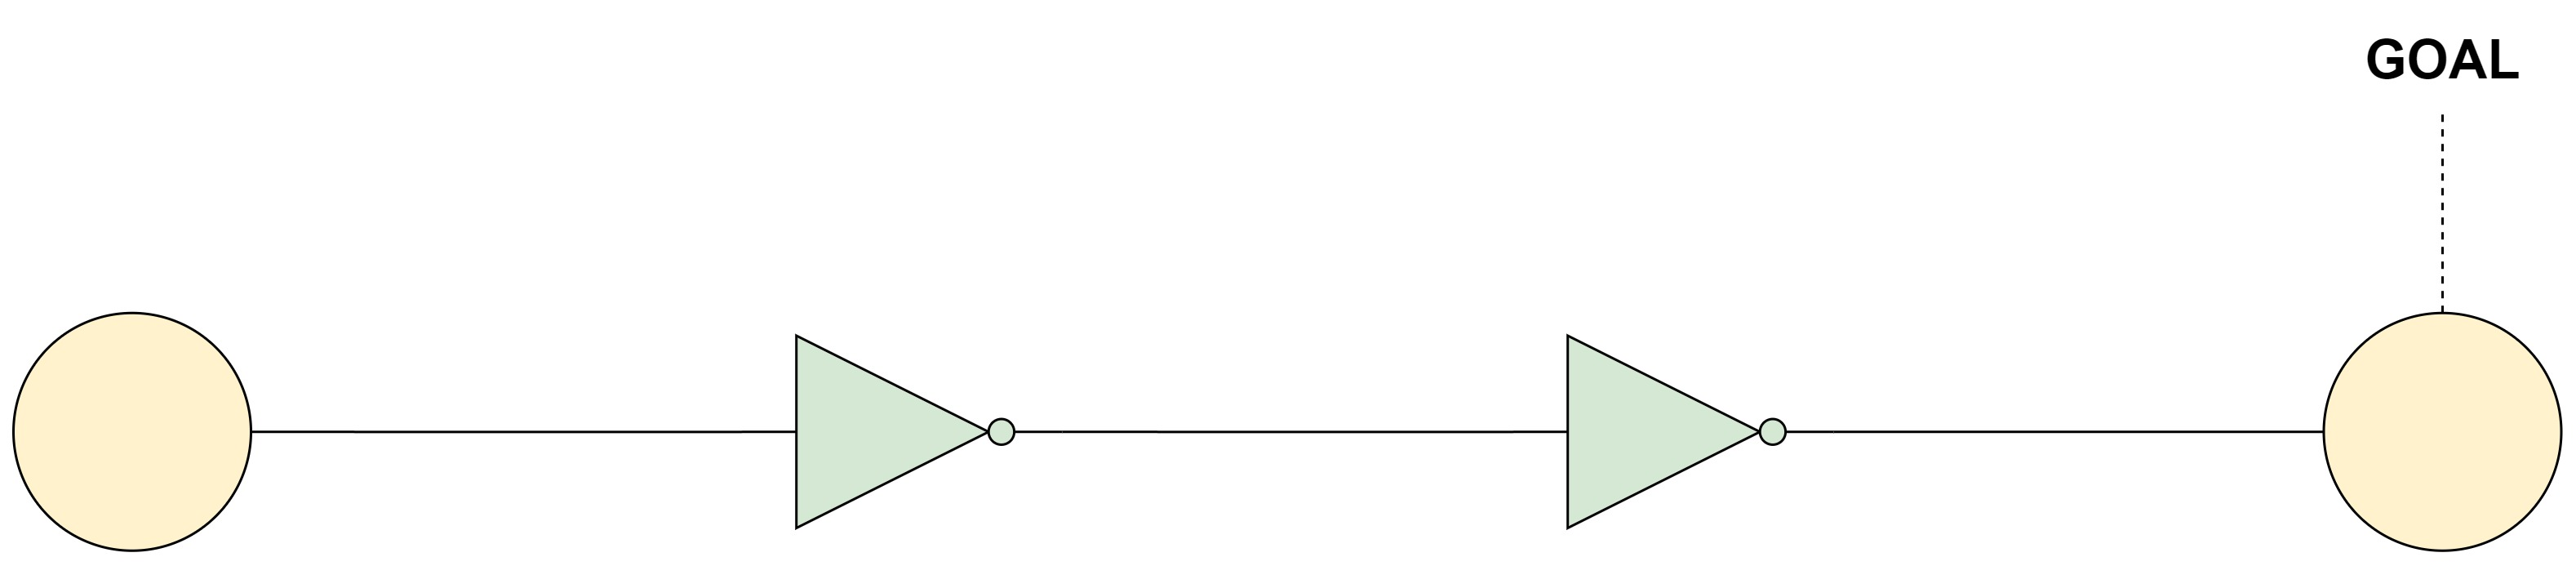
\includegraphics[width=\textwidth]{img/Levels-NOT-1.jpg}
    \caption{Premier Niveau de la porte NOT}
\end{figure}

\begin{figure}[h]
    \centering
    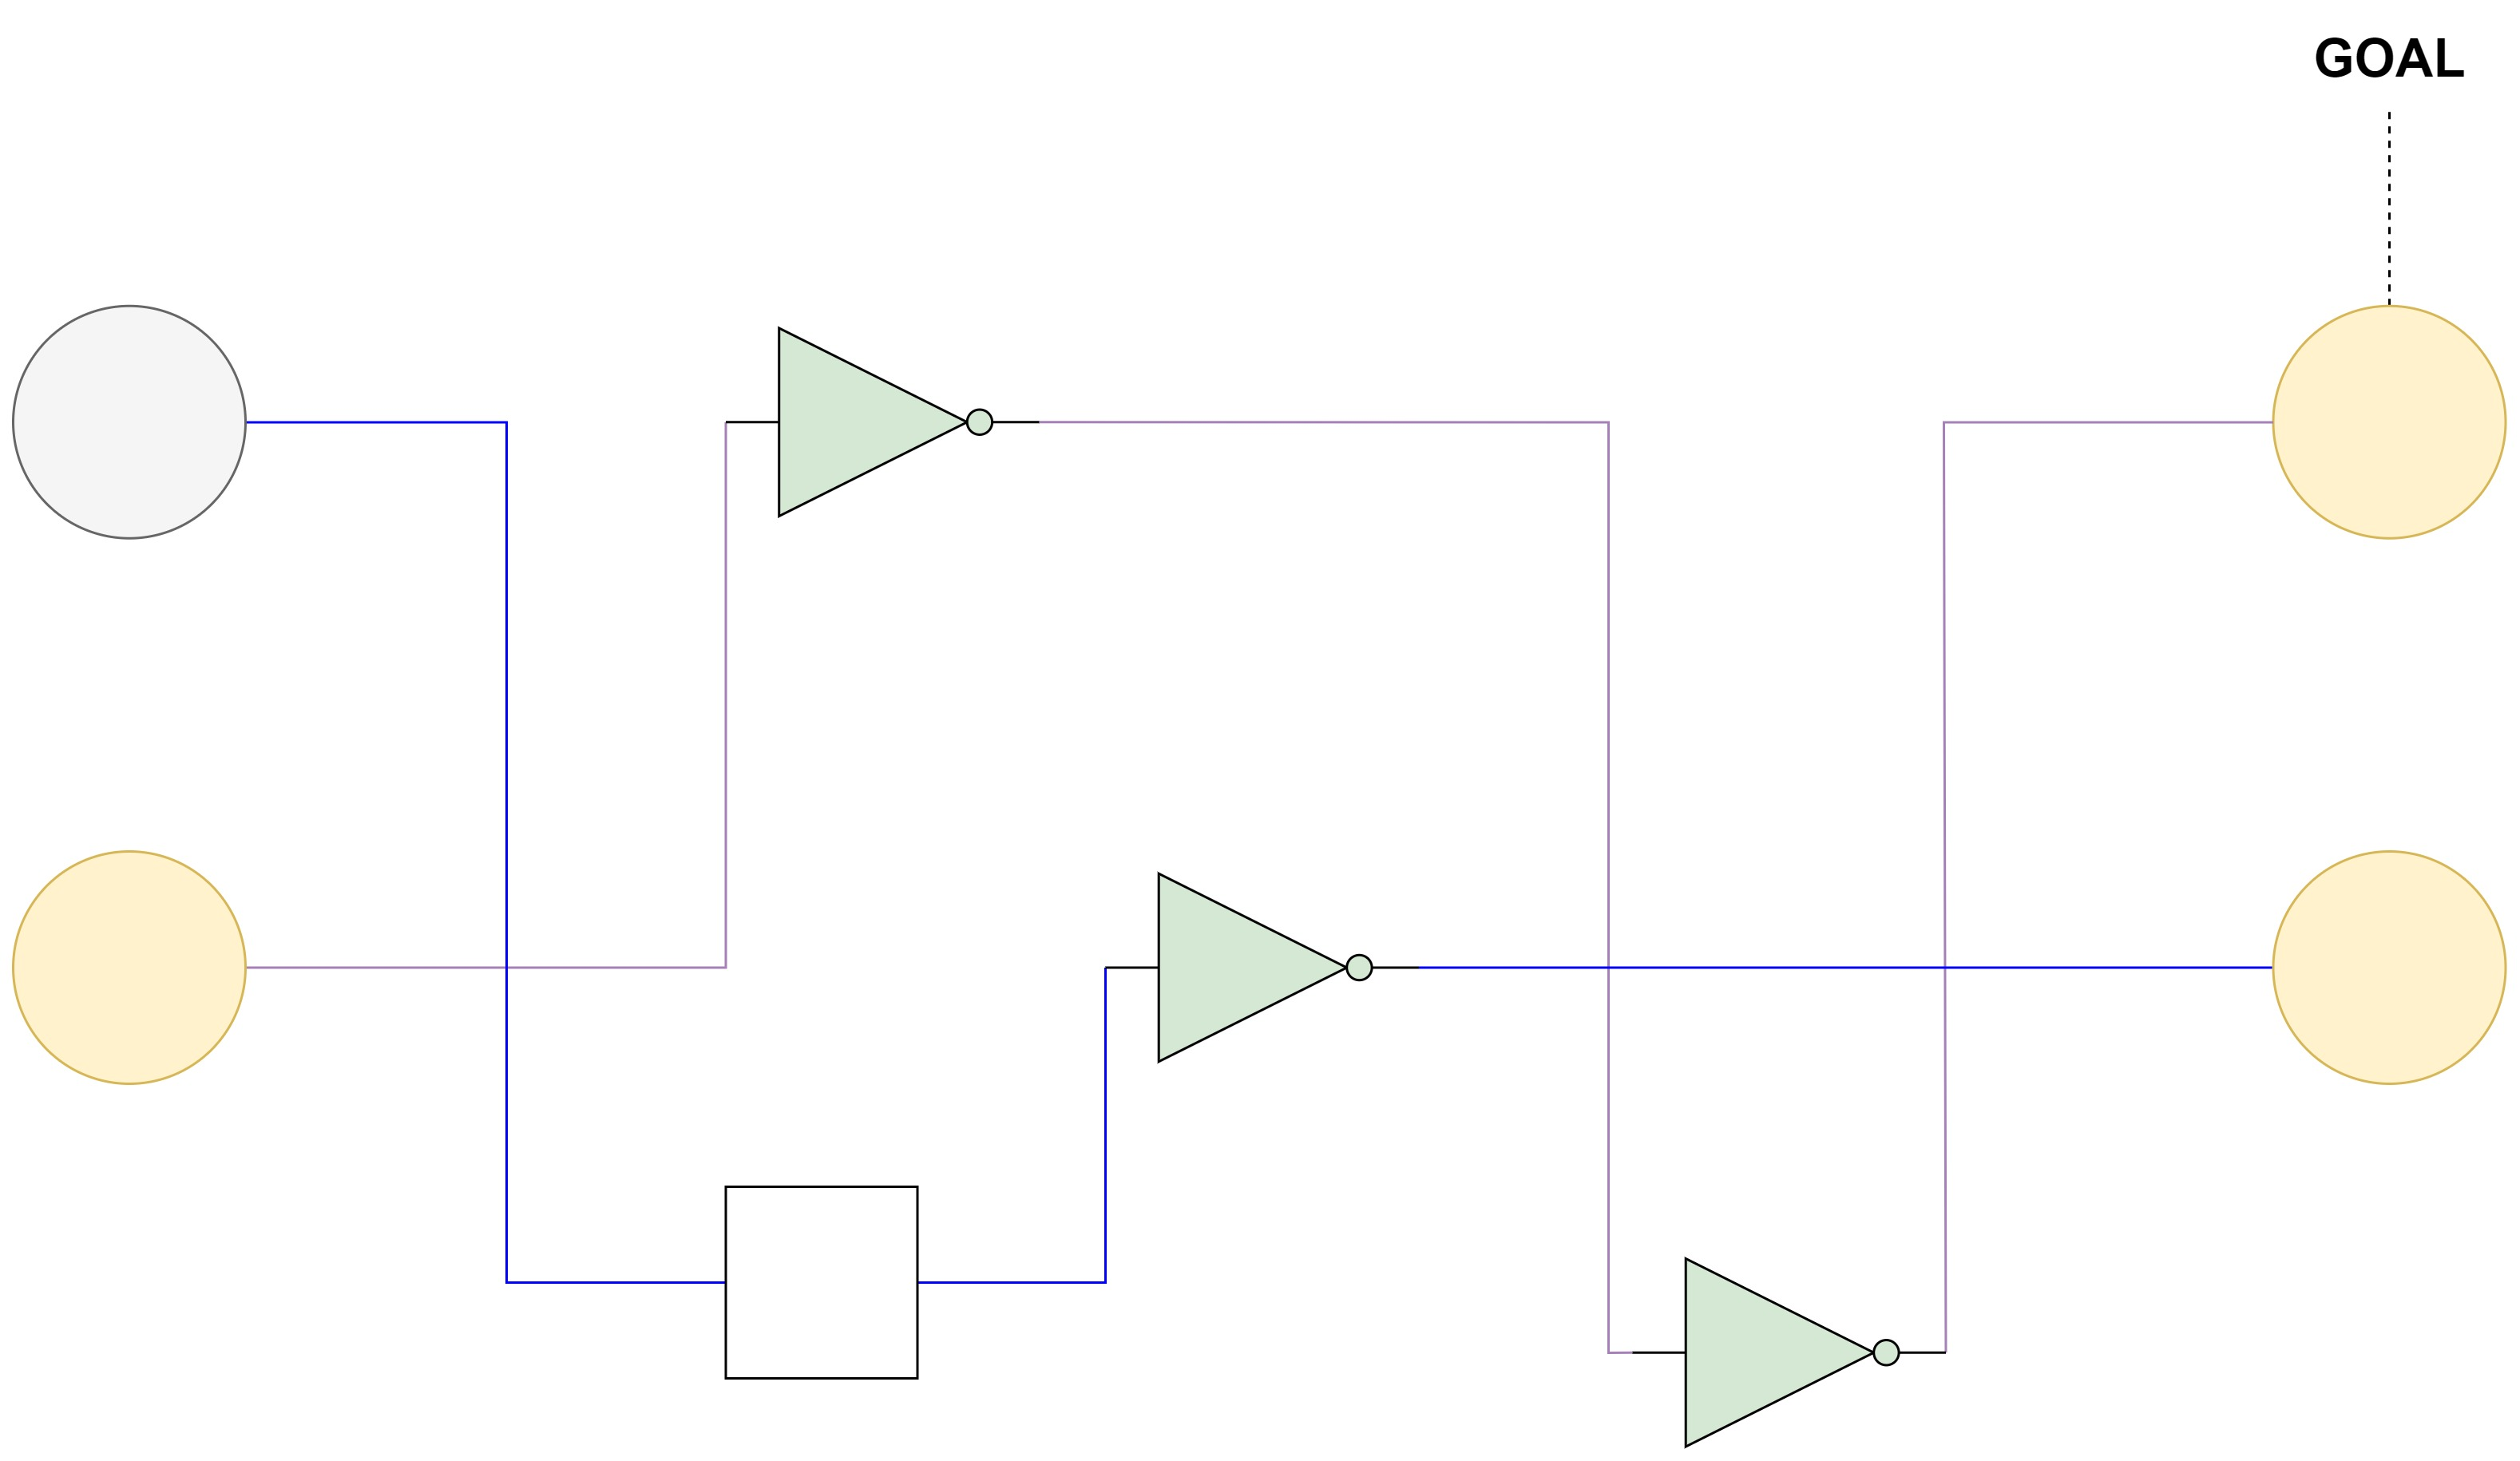
\includegraphics[width=\textwidth]{img/Levels-NOT-2.jpg}
    \caption{2ème Niveau de la porte NOT}
\end{figure}
\begin{figure}[h]
    \centering
    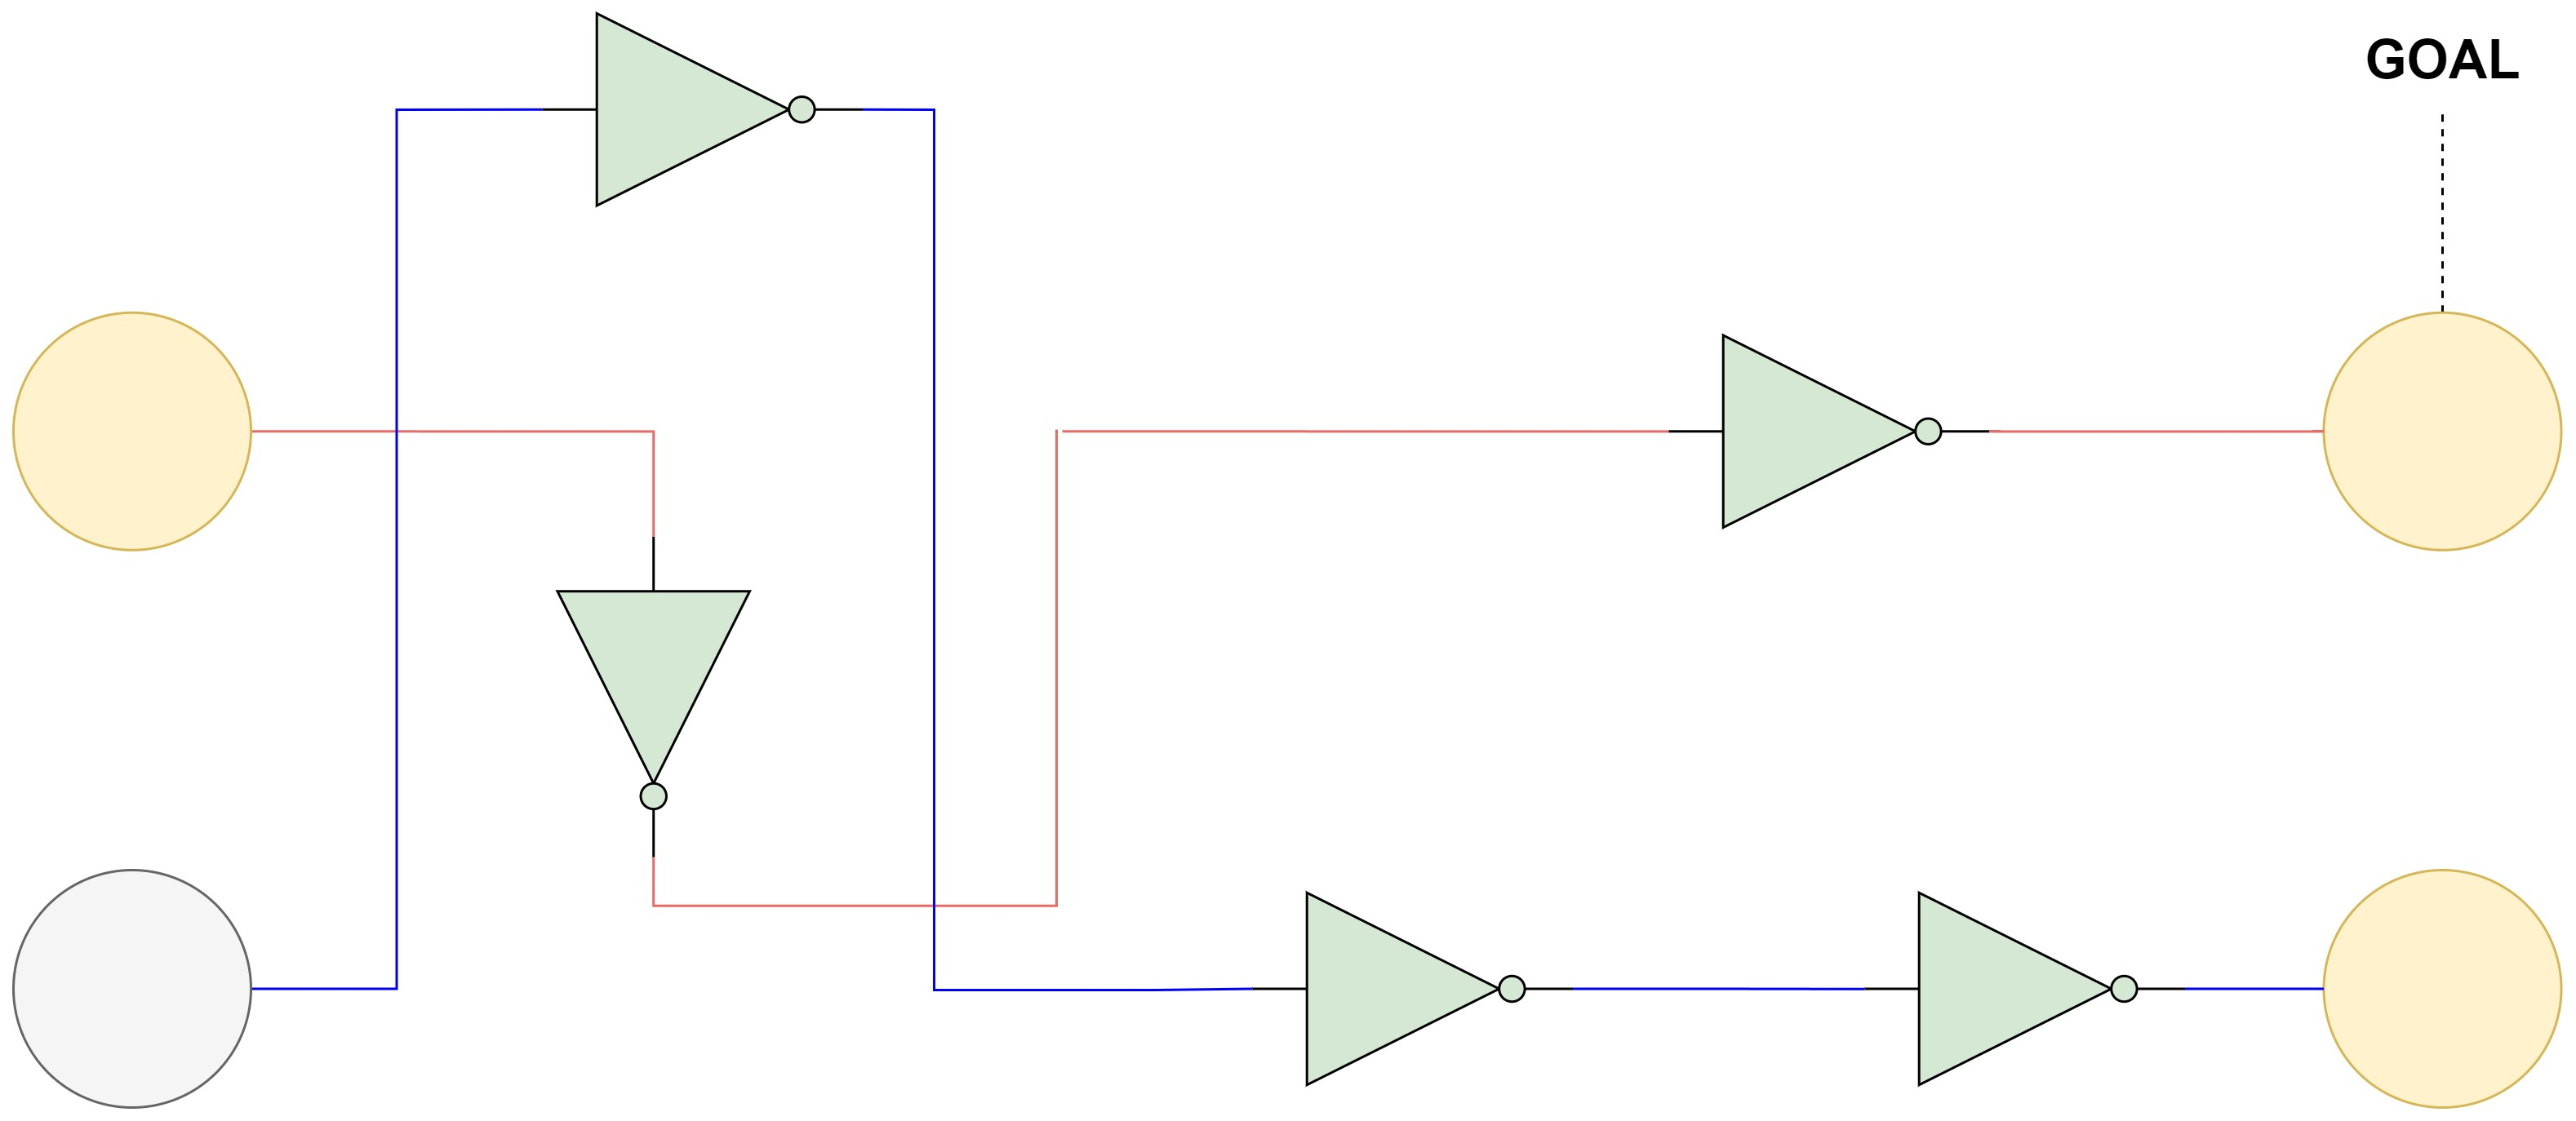
\includegraphics[width=\textwidth]{img/Levels-NOT-3.jpg}
    \caption{3ème Niveau de la porte NOT}
\end{figure}
\begin{figure}[h]
    \centering
    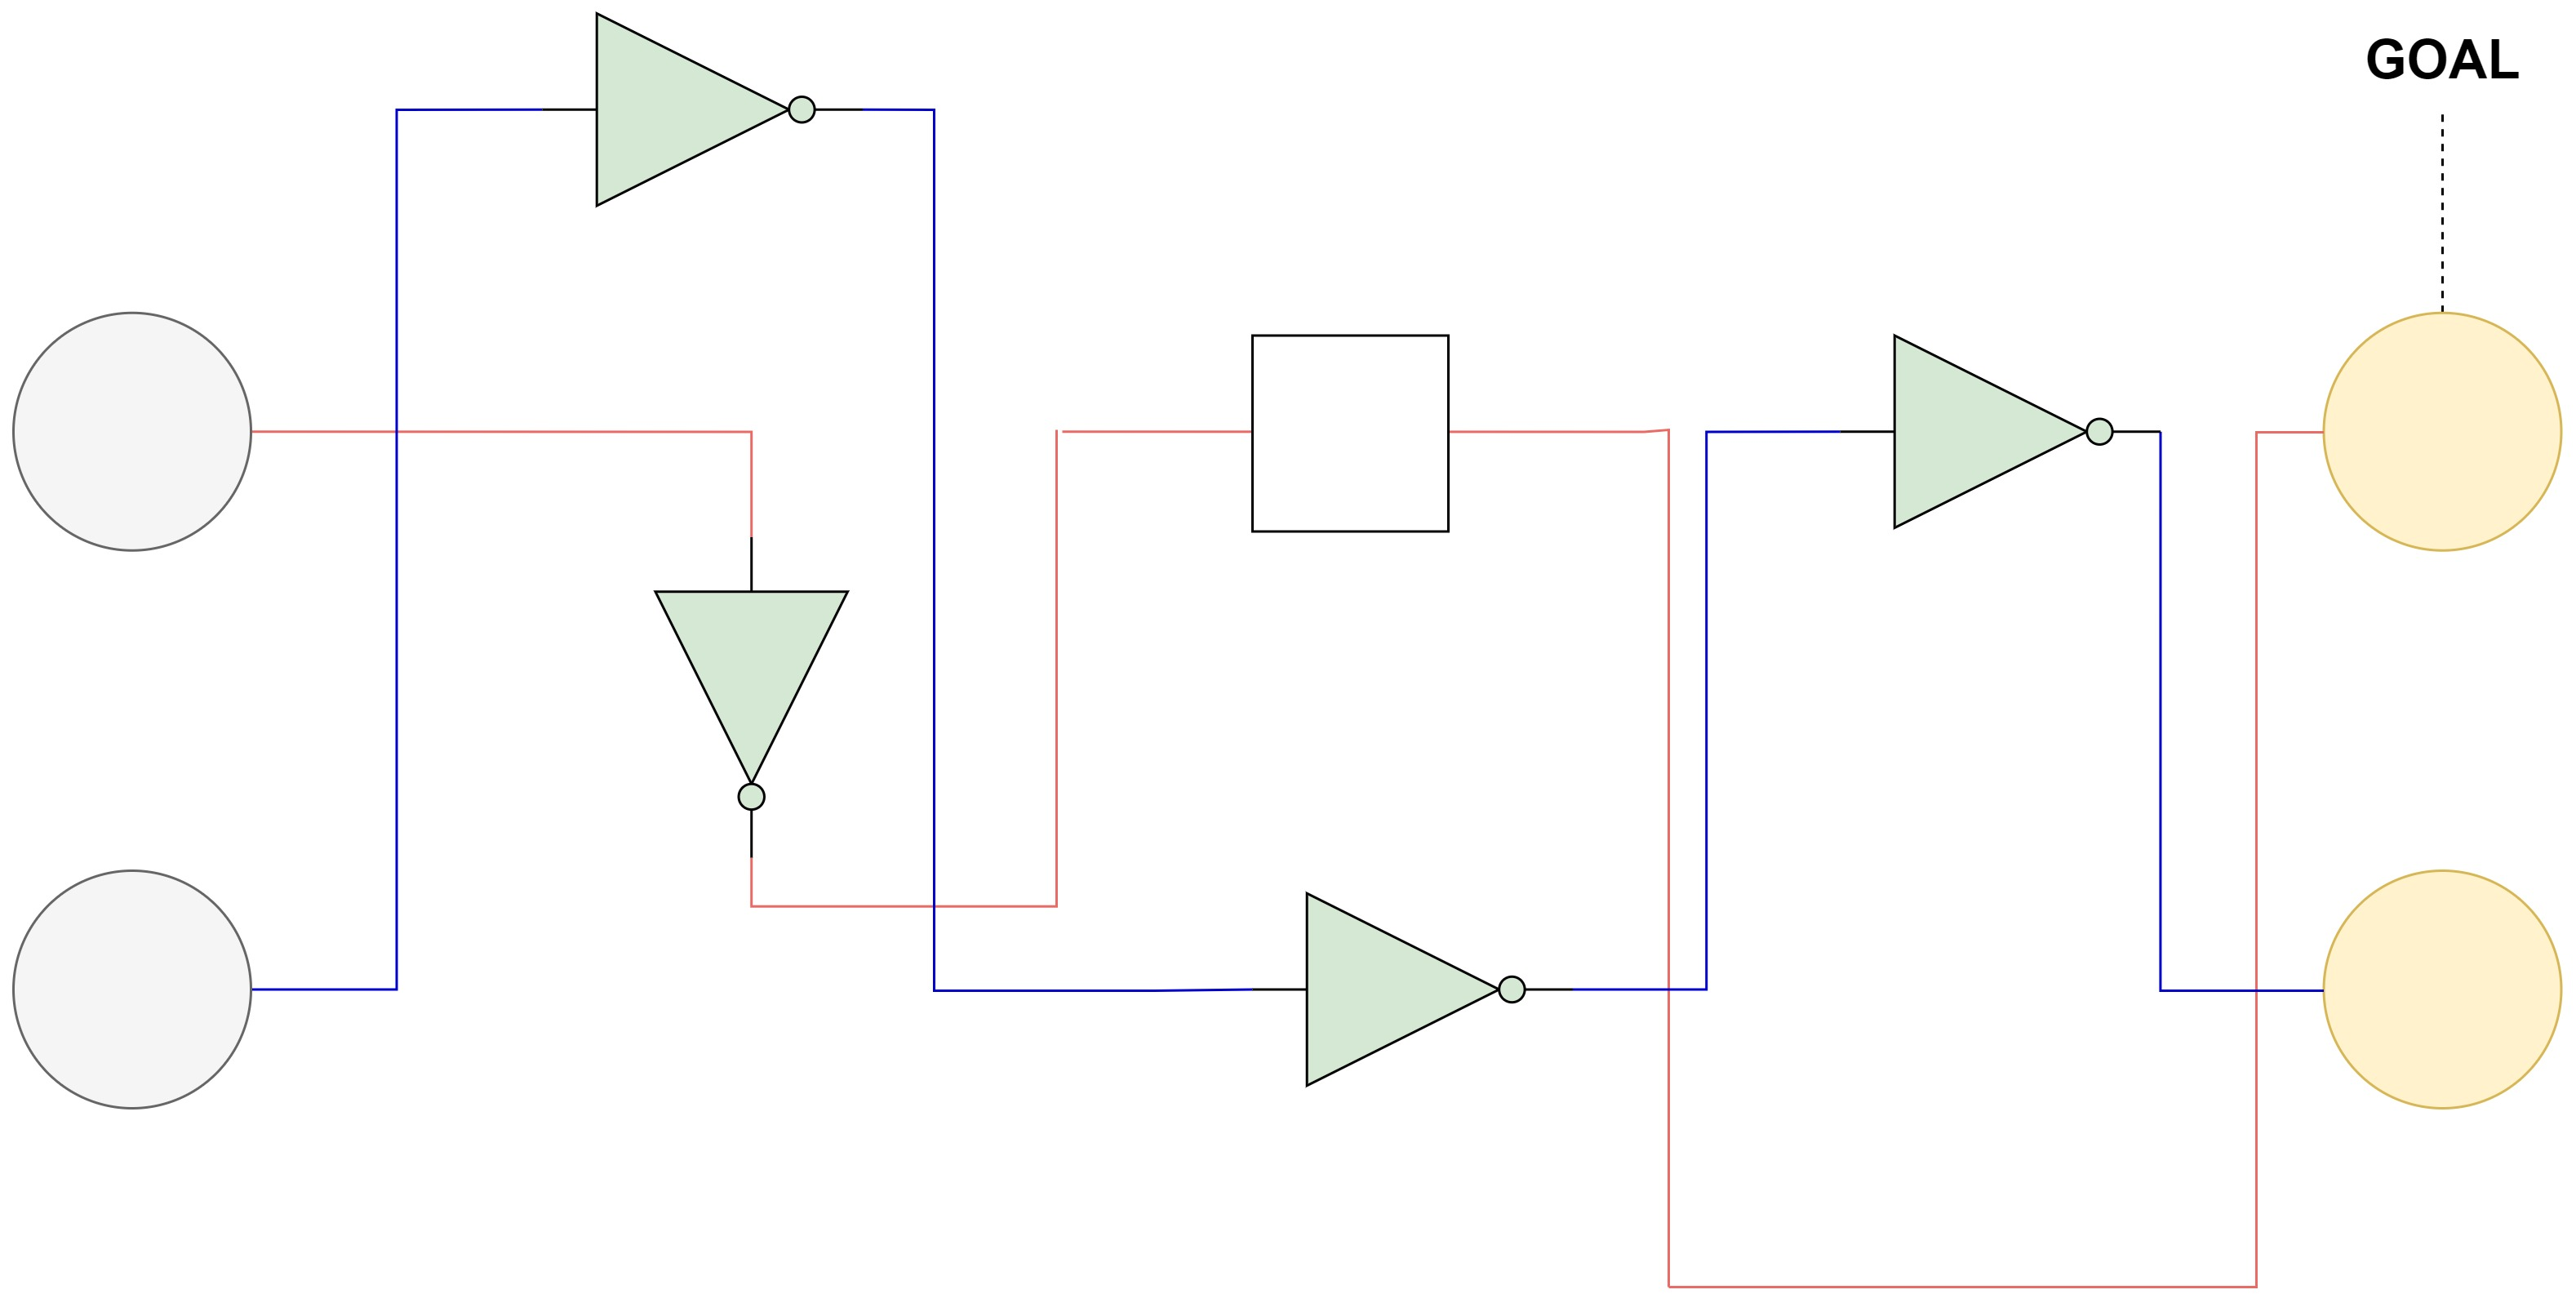
\includegraphics[width=\textwidth]{img/Levels-NOT-4.jpg}
    \caption{4ème Niveau de la porte NOT}
\end{figure}
\begin{figure}[h]
    \centering
    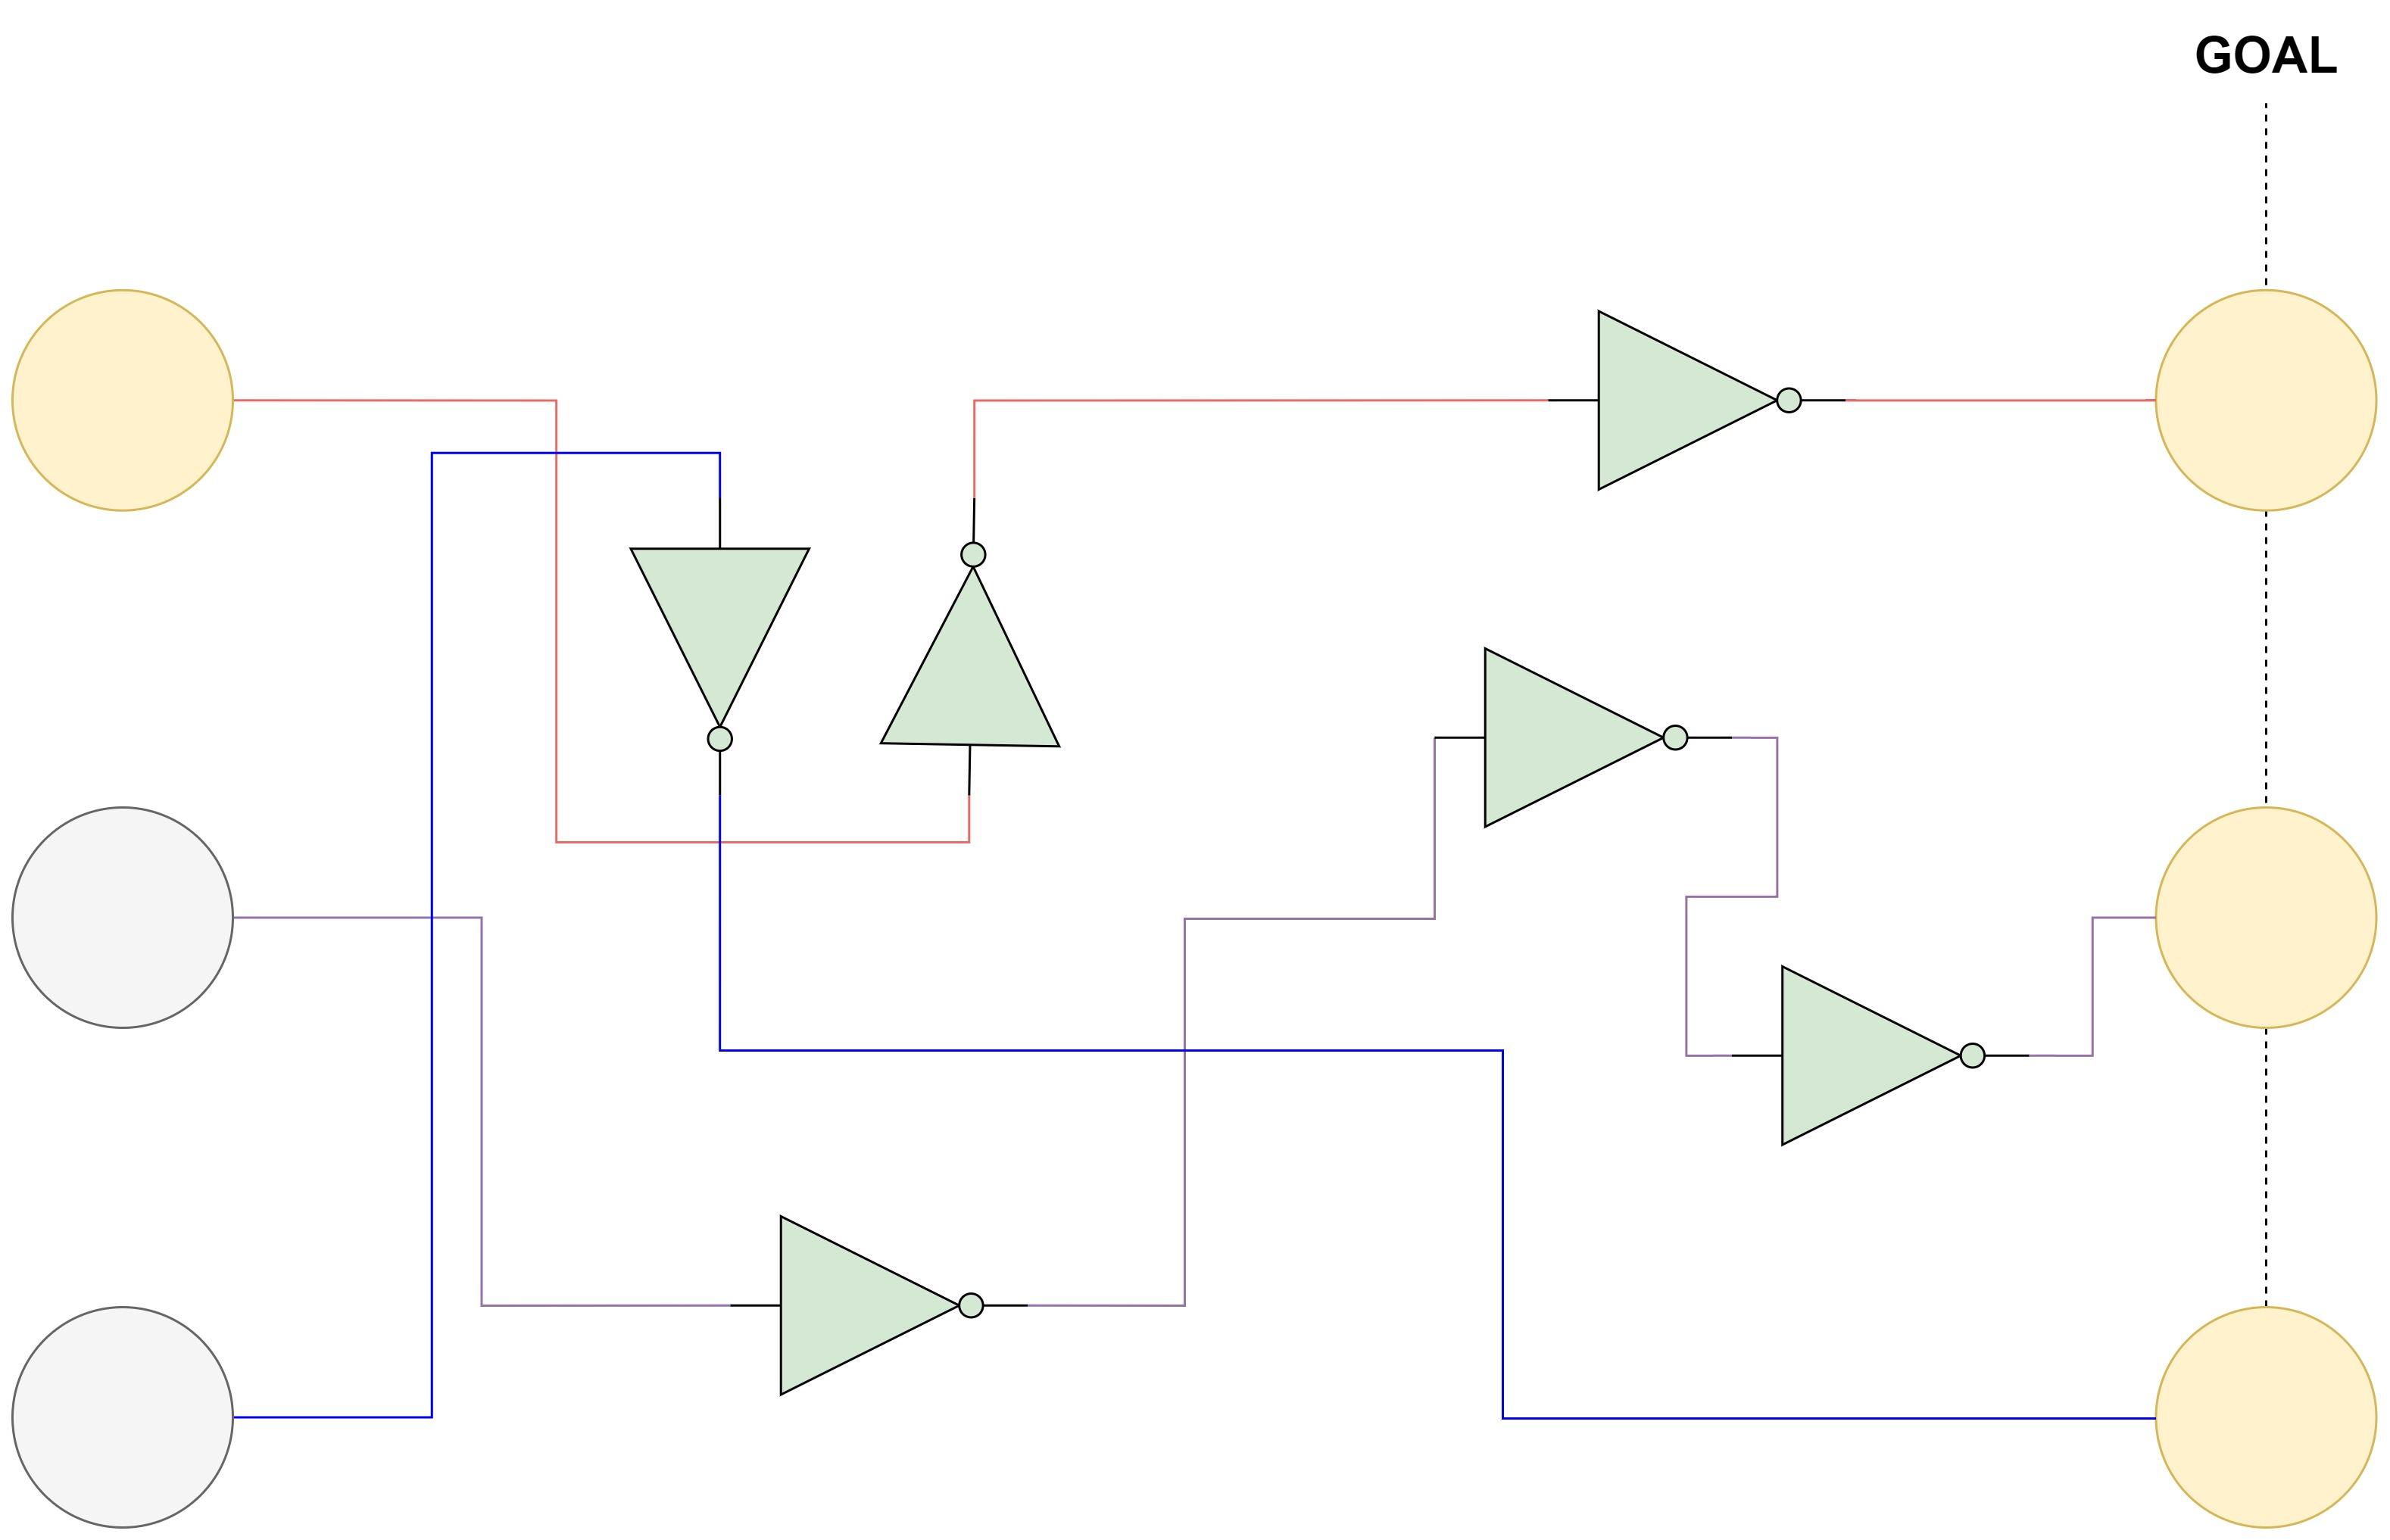
\includegraphics[width=\textwidth]{img/Levels-NOT-5.jpg}
    \caption{5ème Niveau de la porte NOT}
\end{figure}
\begin{figure}[h]
    \centering
    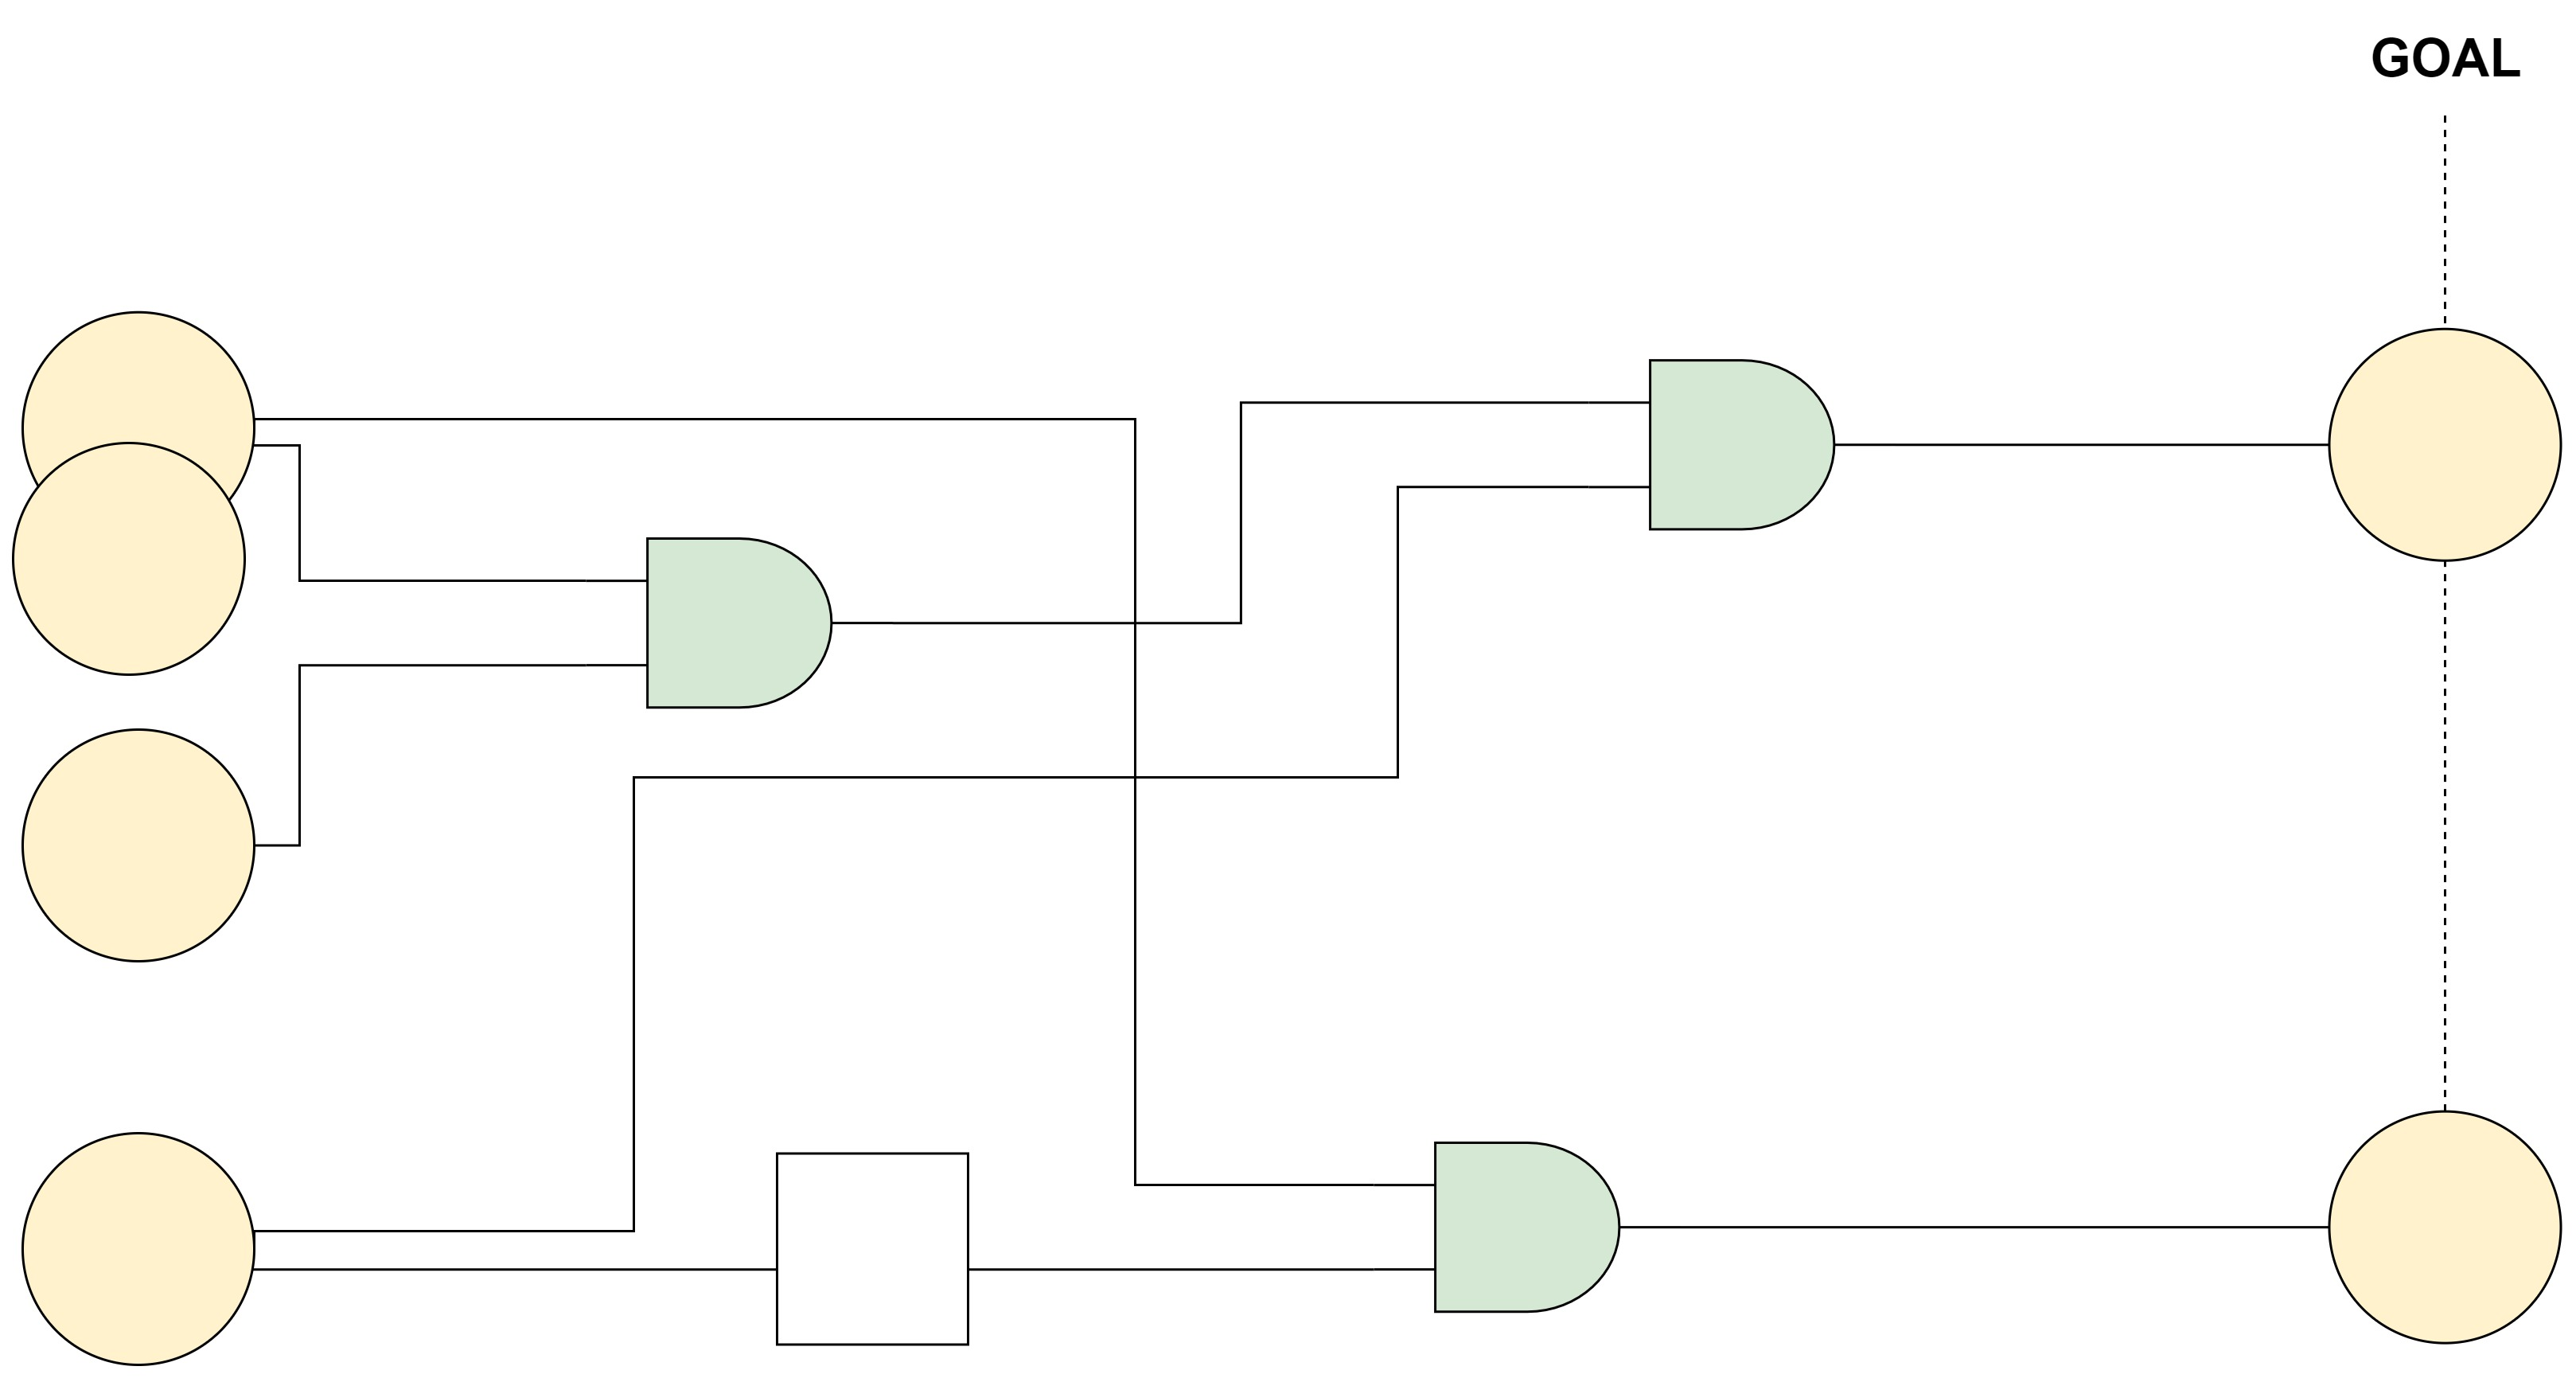
\includegraphics[width=\textwidth]{img/Levels-AND-1.jpg}
    \caption{Premier Niveau de la porte AND}
\end{figure}
\begin{figure}[h]
    \centering
    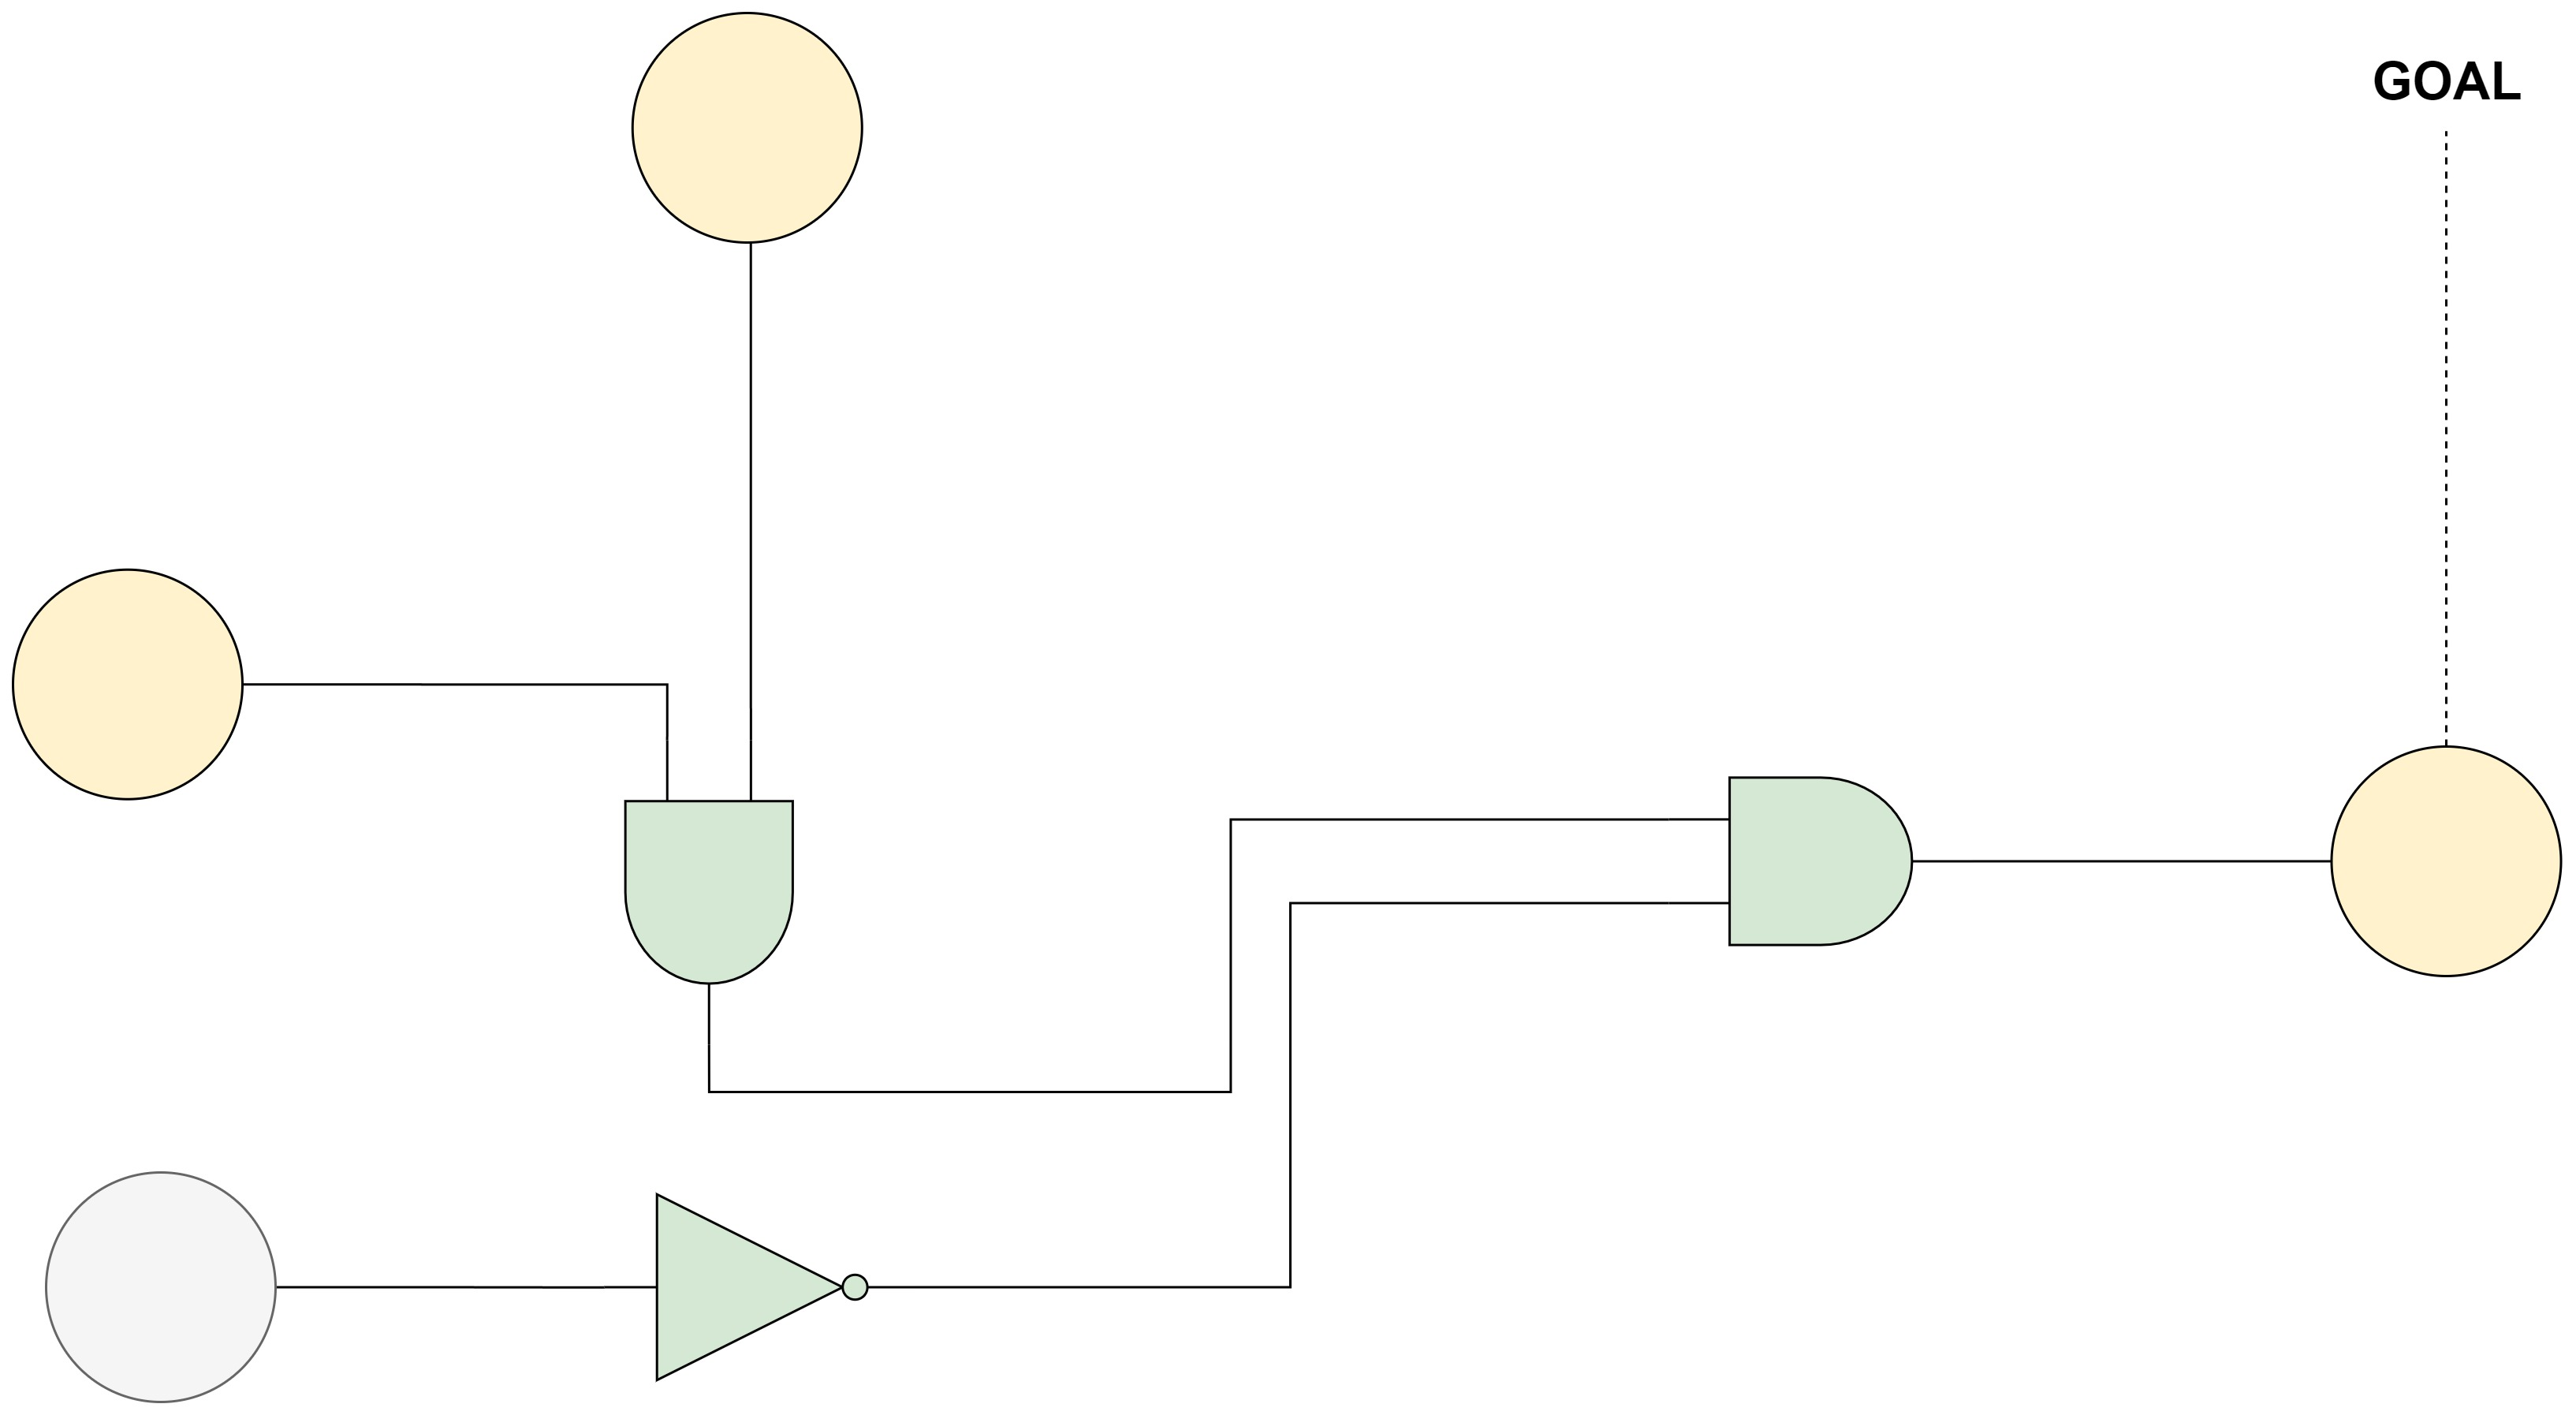
\includegraphics[width=\textwidth]{img/Levels-AND-2.jpg}
    \caption{2ème Niveau de la porte AND}
\end{figure}
\begin{figure}[h]
    \centering
    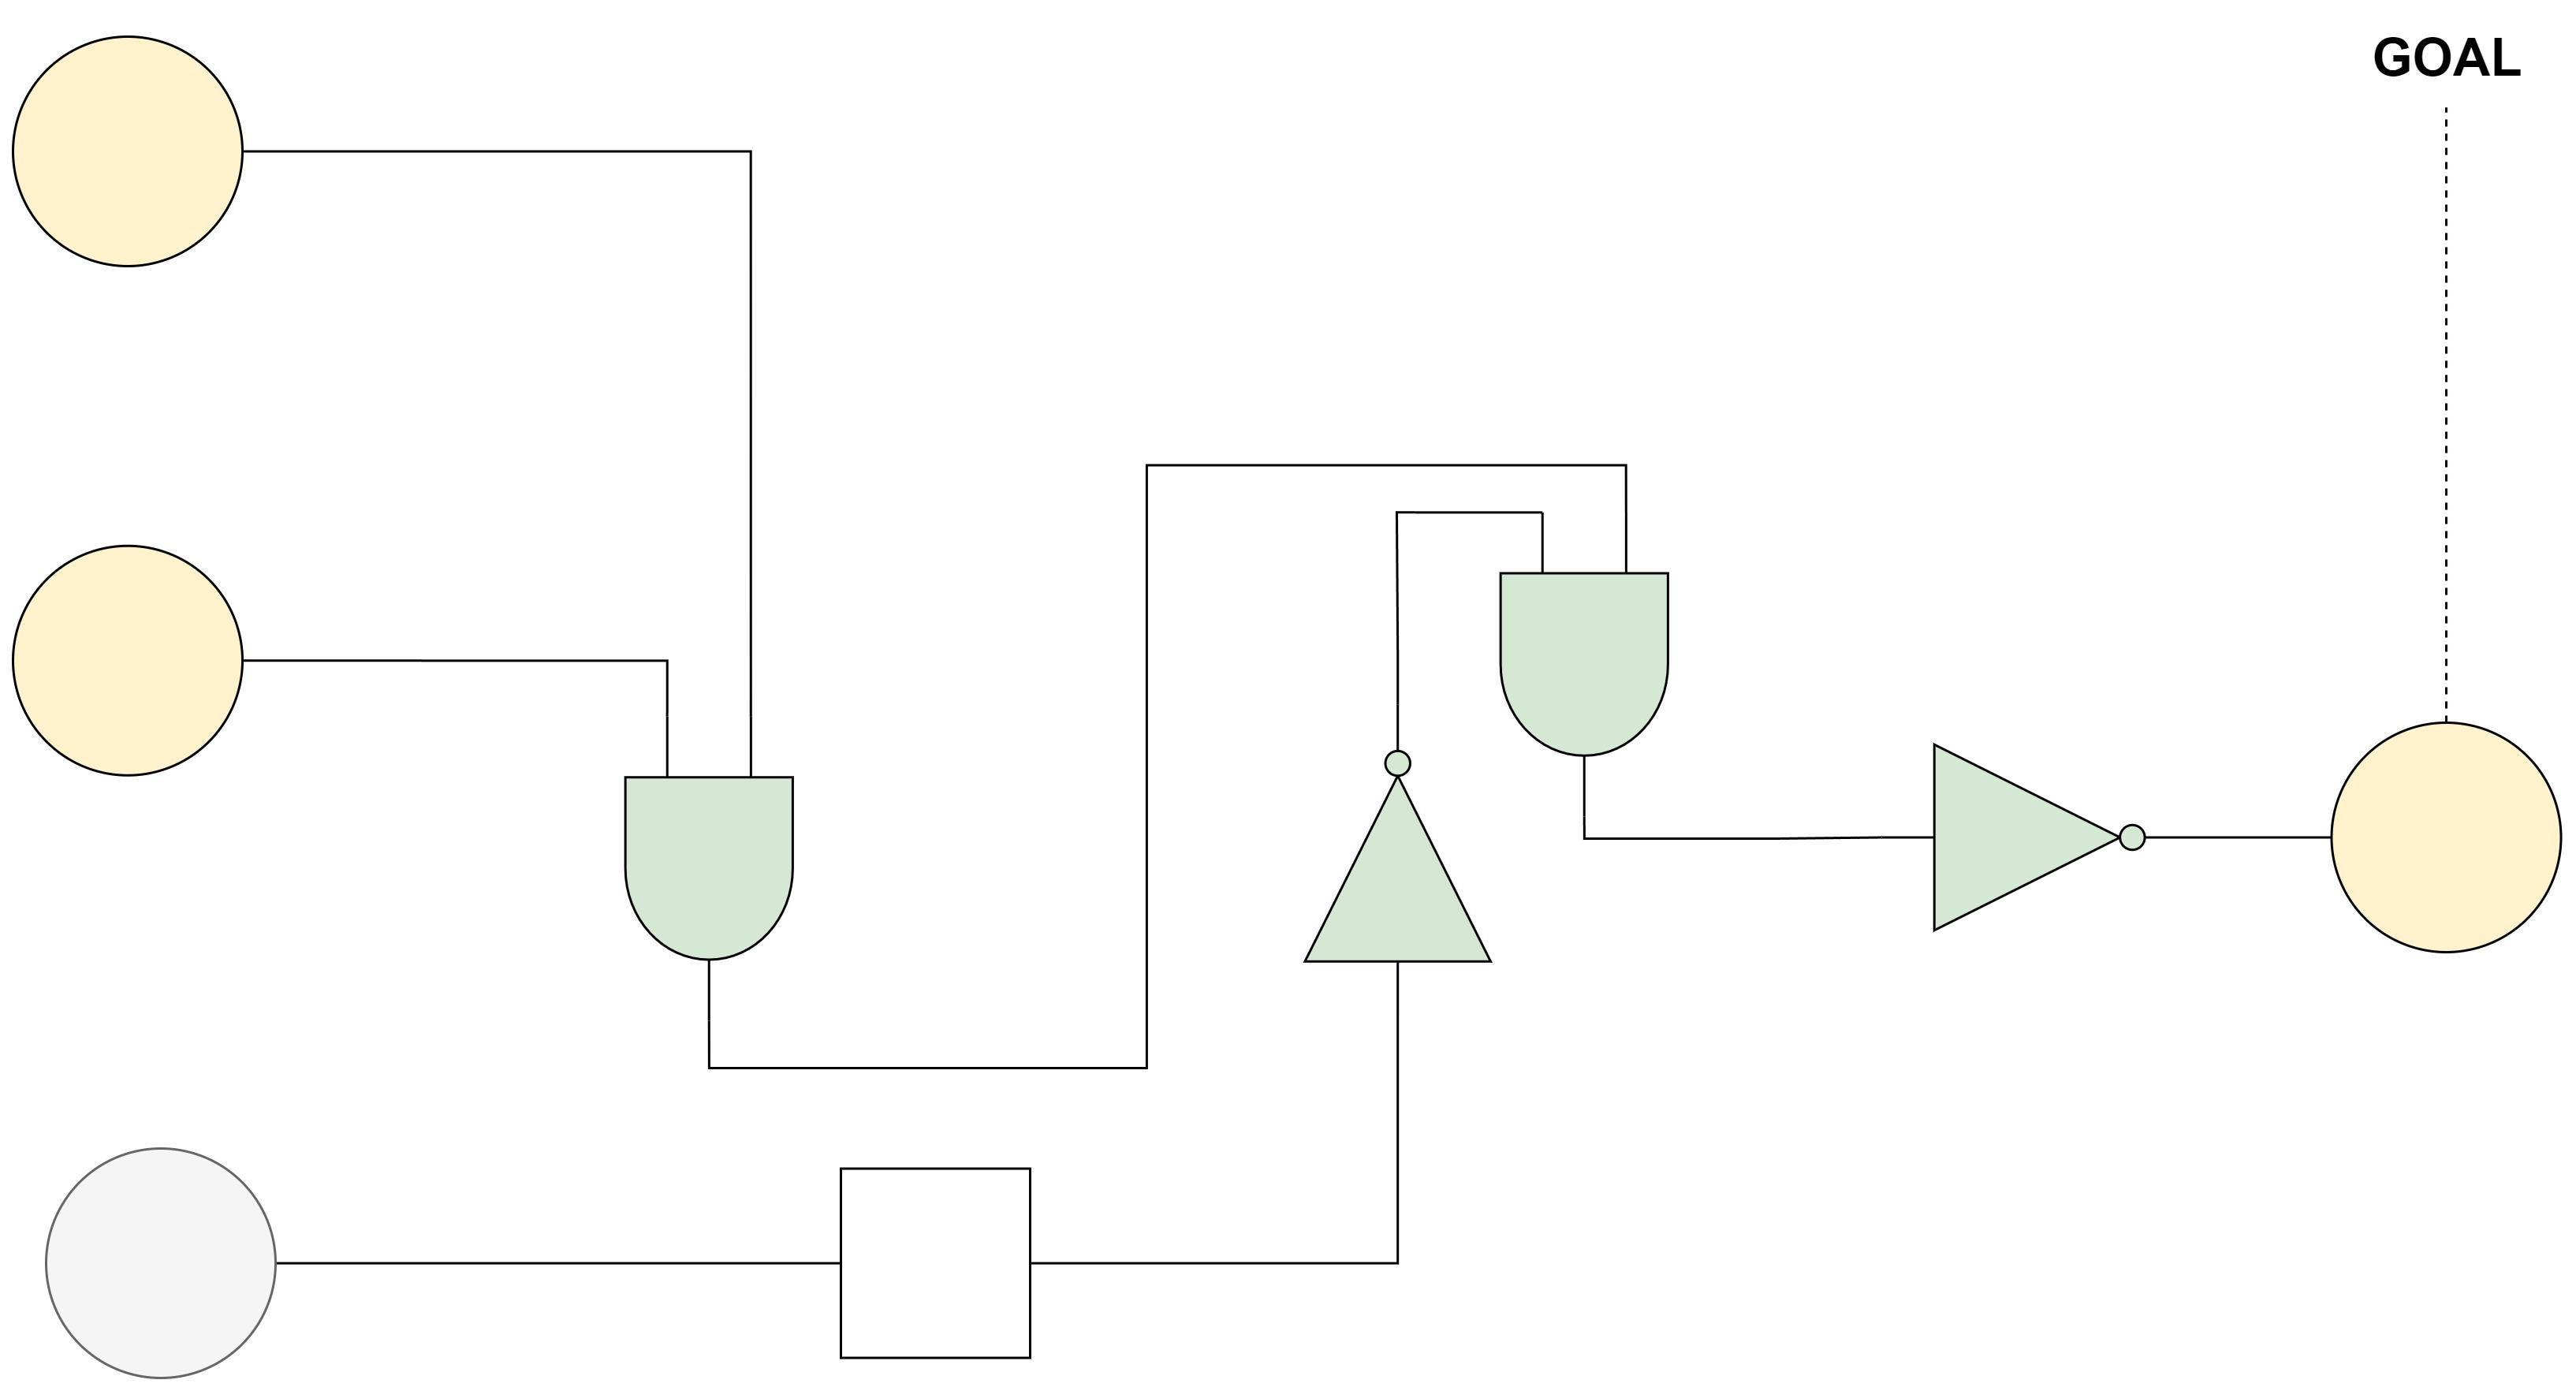
\includegraphics[width=\textwidth]{img/Levels-AND-3.jpg}
    \caption{3ème Niveau de la porte AND}
\end{figure}
\begin{figure}[h]
    \centering
    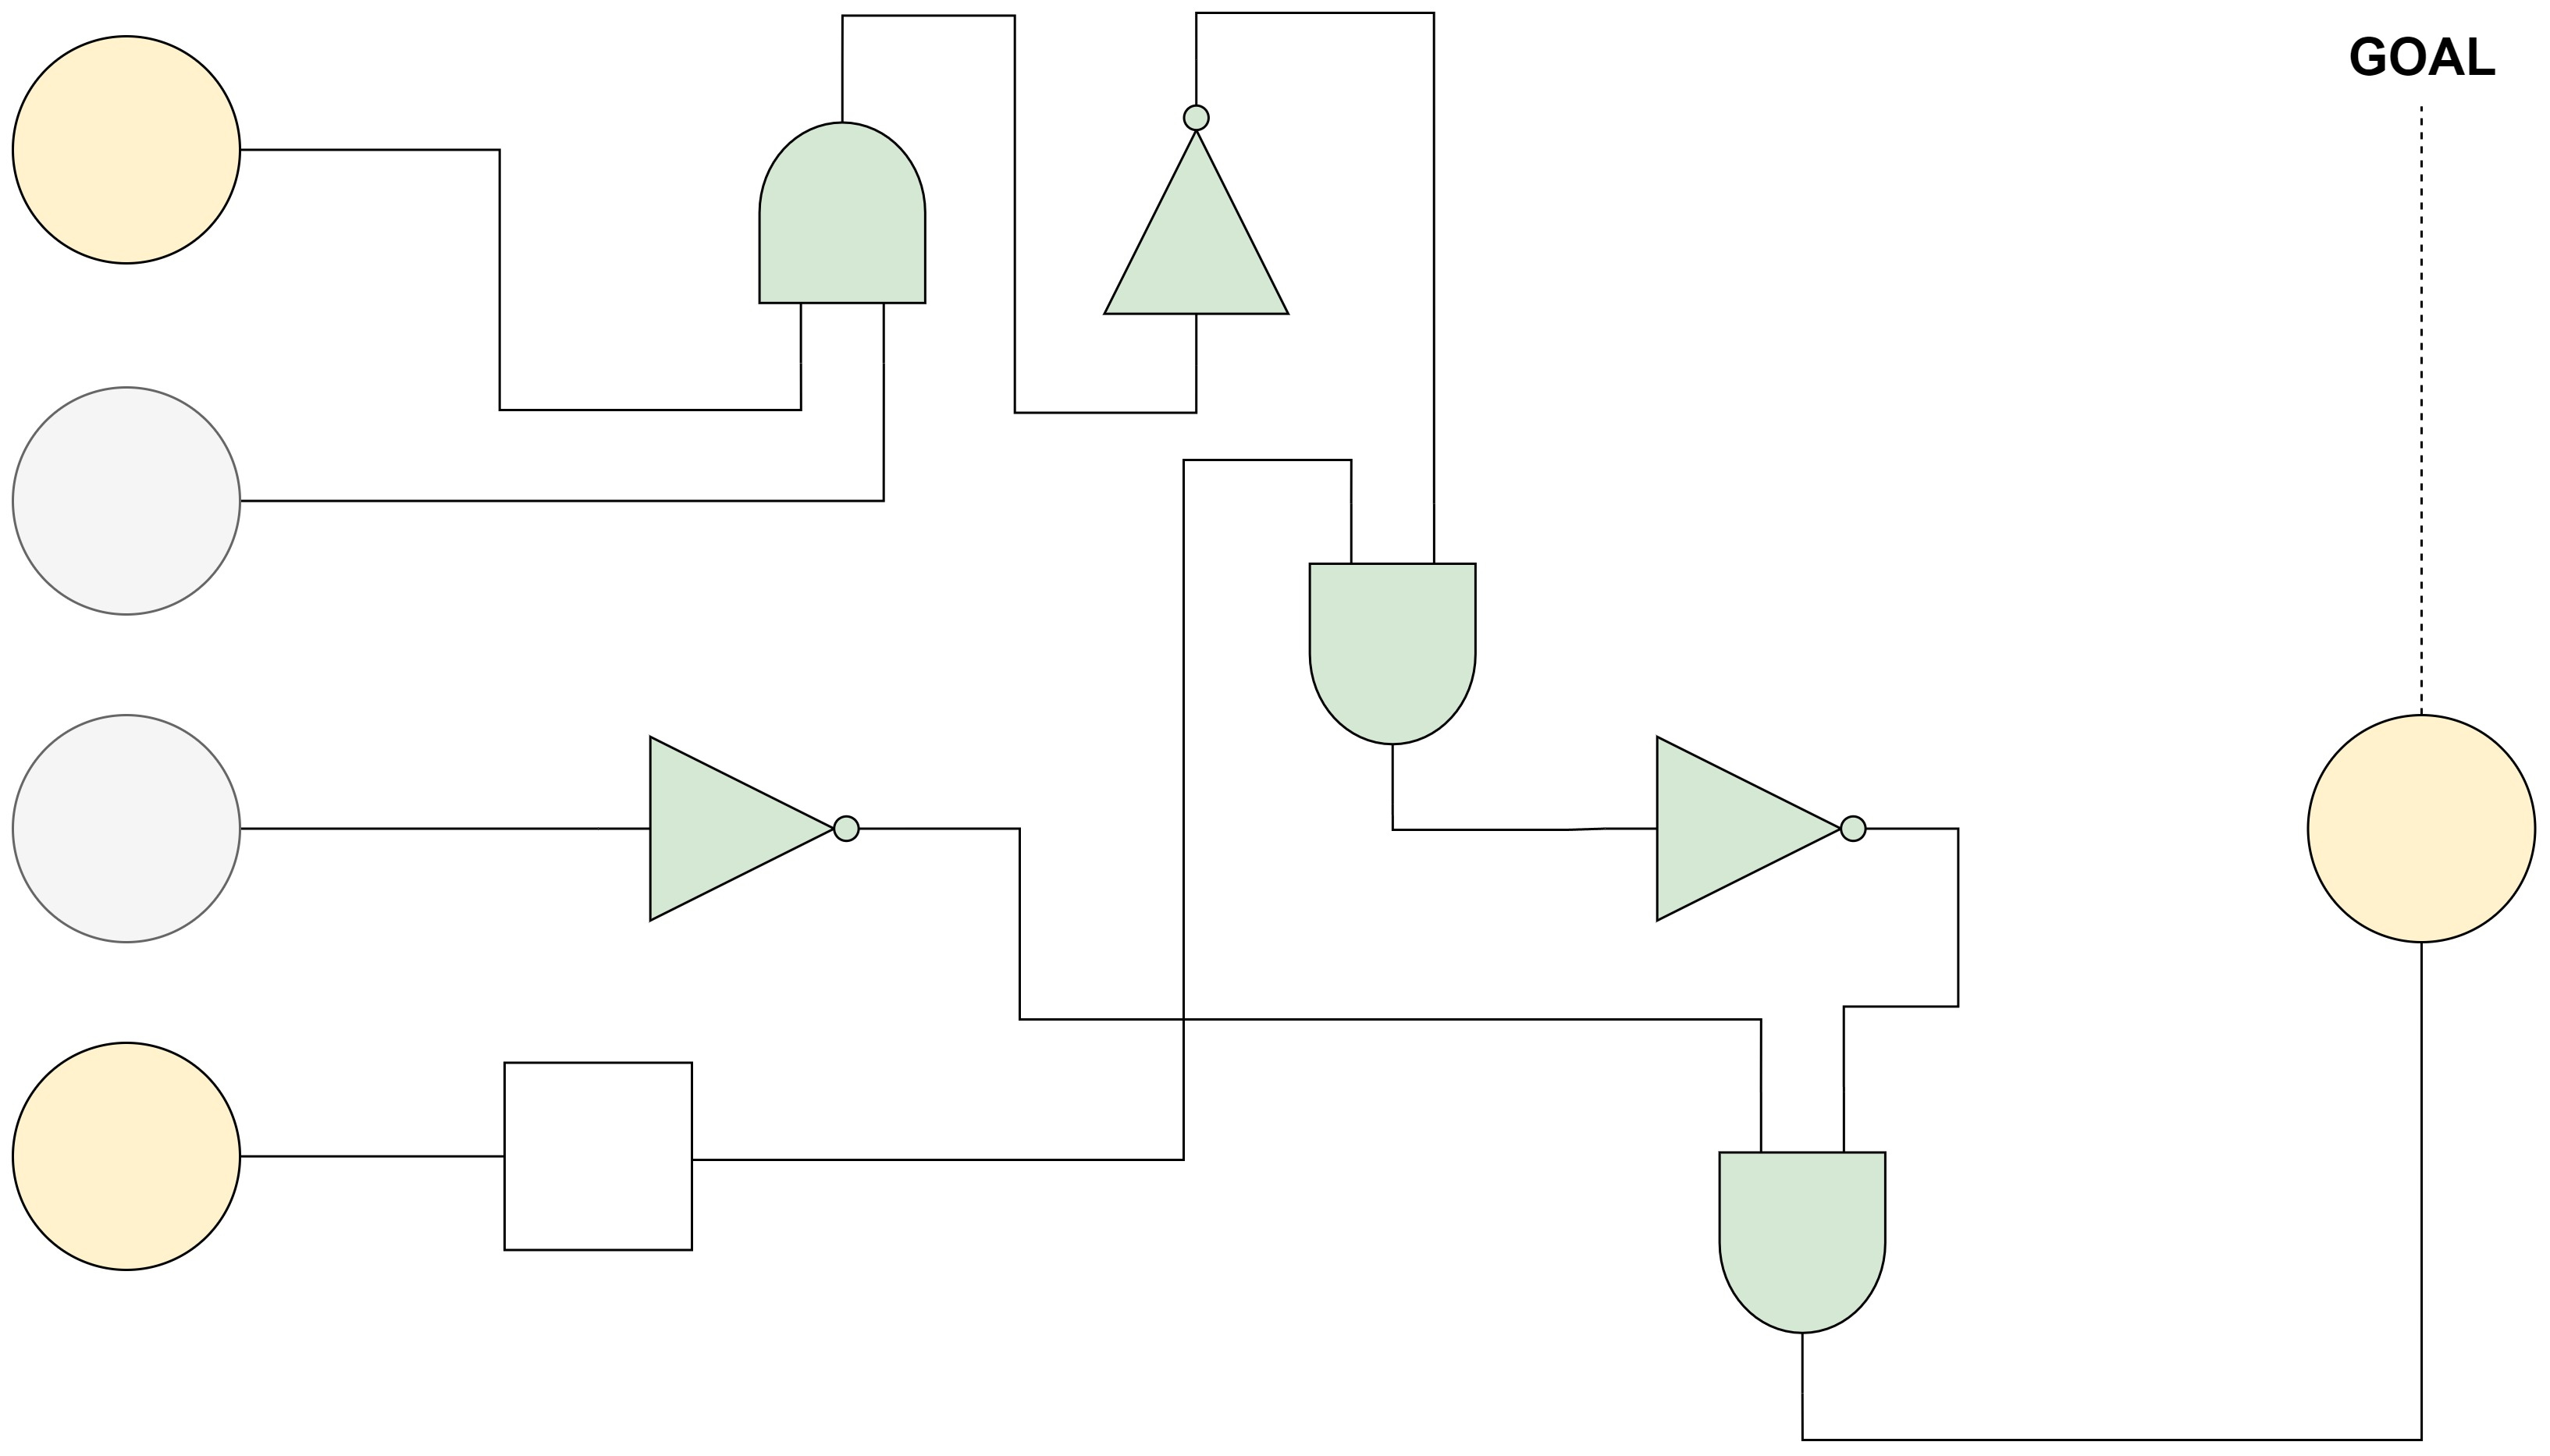
\includegraphics[width=\textwidth]{img/Levels-AND-4.jpg}
    \caption{4ème Niveau de la porte AND}
\end{figure}
\begin{figure}[h]
    \centering
    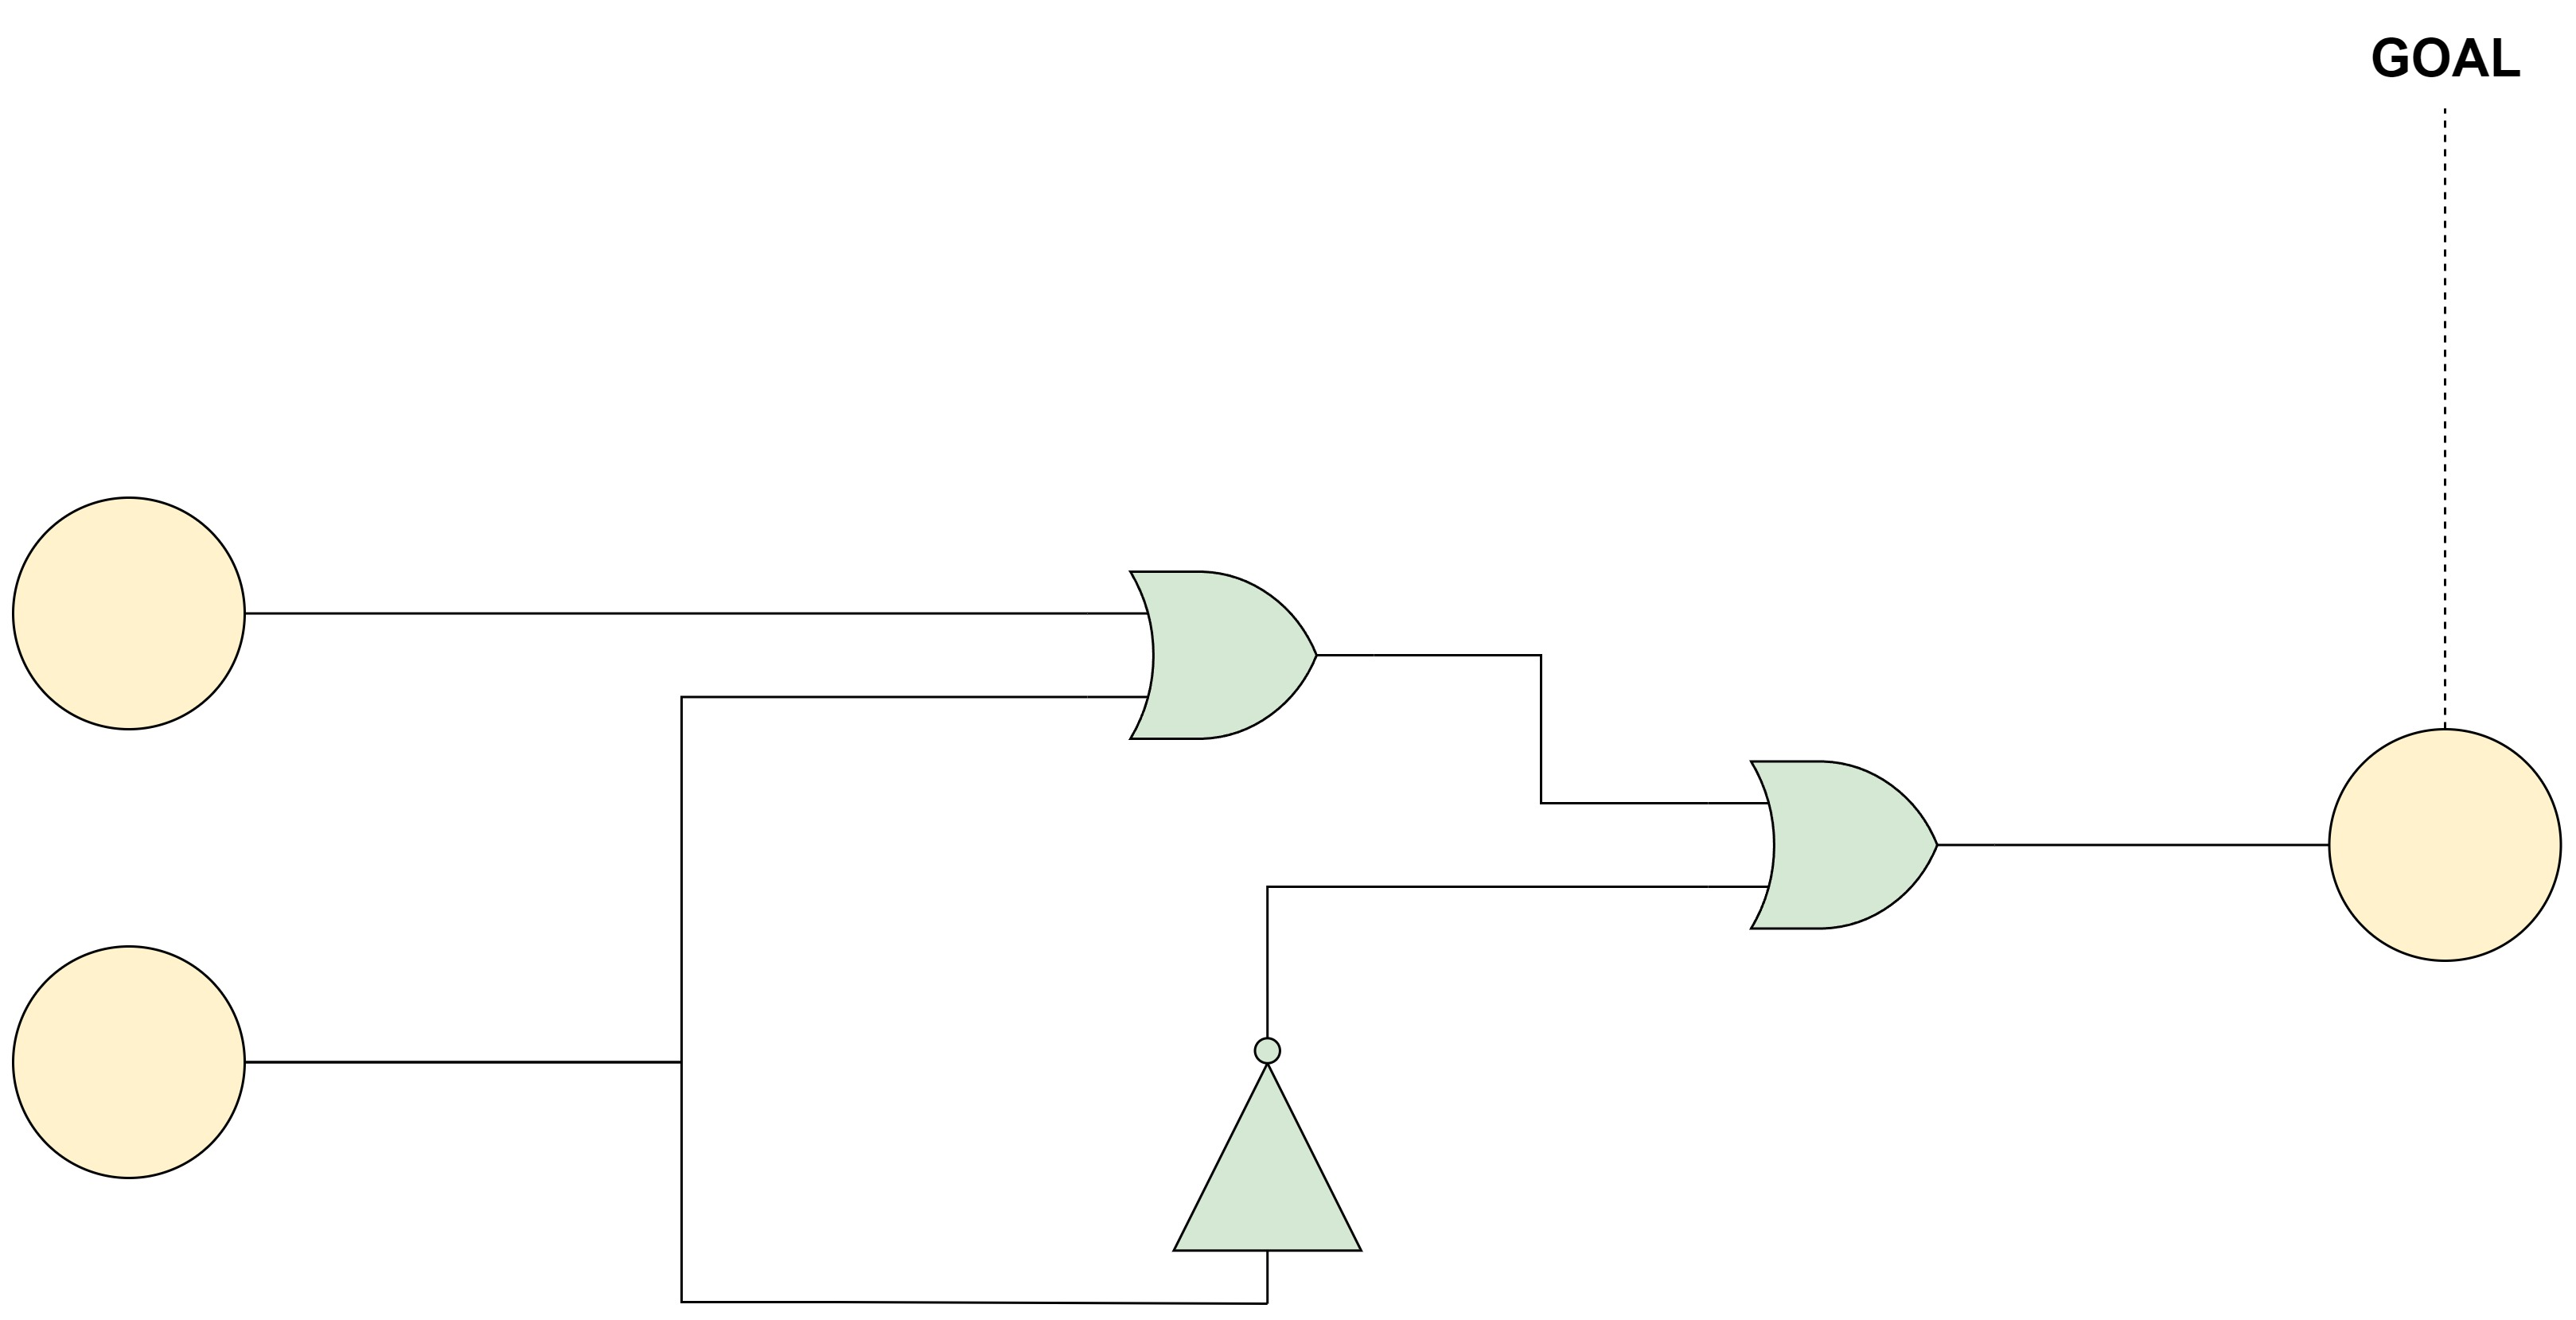
\includegraphics[width=\textwidth]{img/Levels-OR-1.jpg}
    \caption{Premier Niveau de la porte OR}
\end{figure}
\begin{figure}[h]
    \centering
    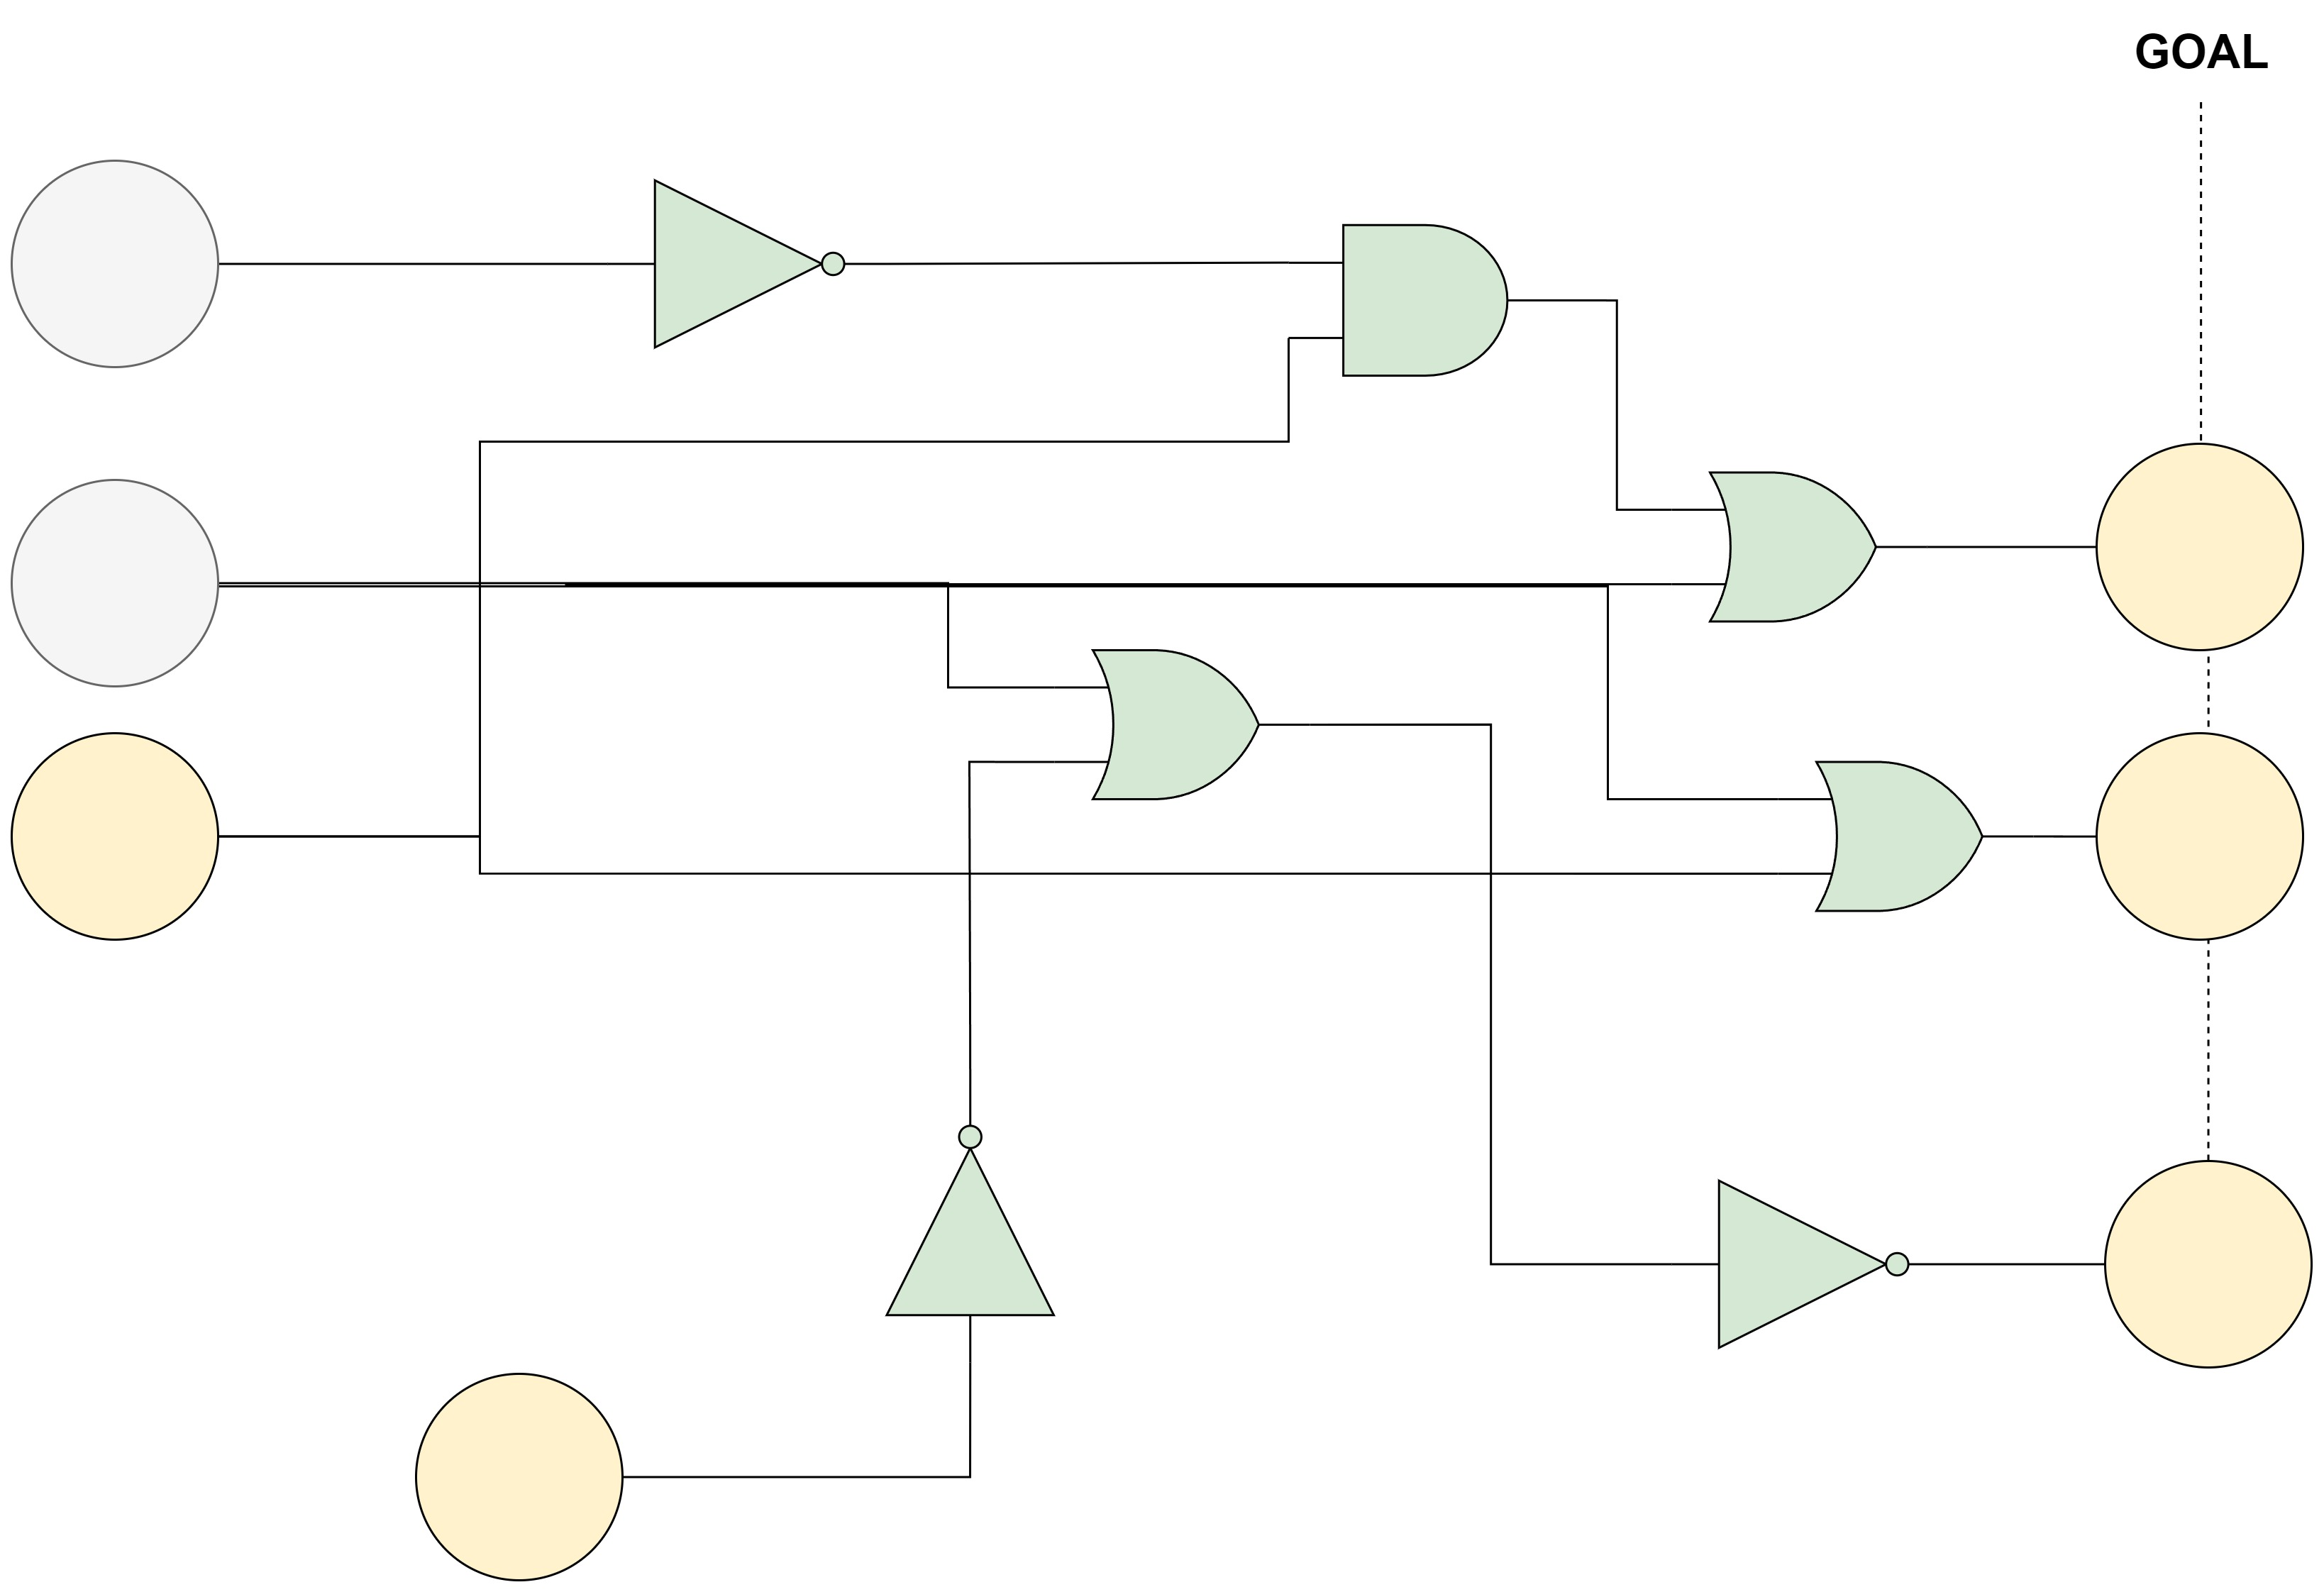
\includegraphics[width=\textwidth]{img/Levels-OR-2.jpg}
    \caption{2ème Niveau de la porte OR}
\end{figure}
\begin{figure}[h]
    \centering
    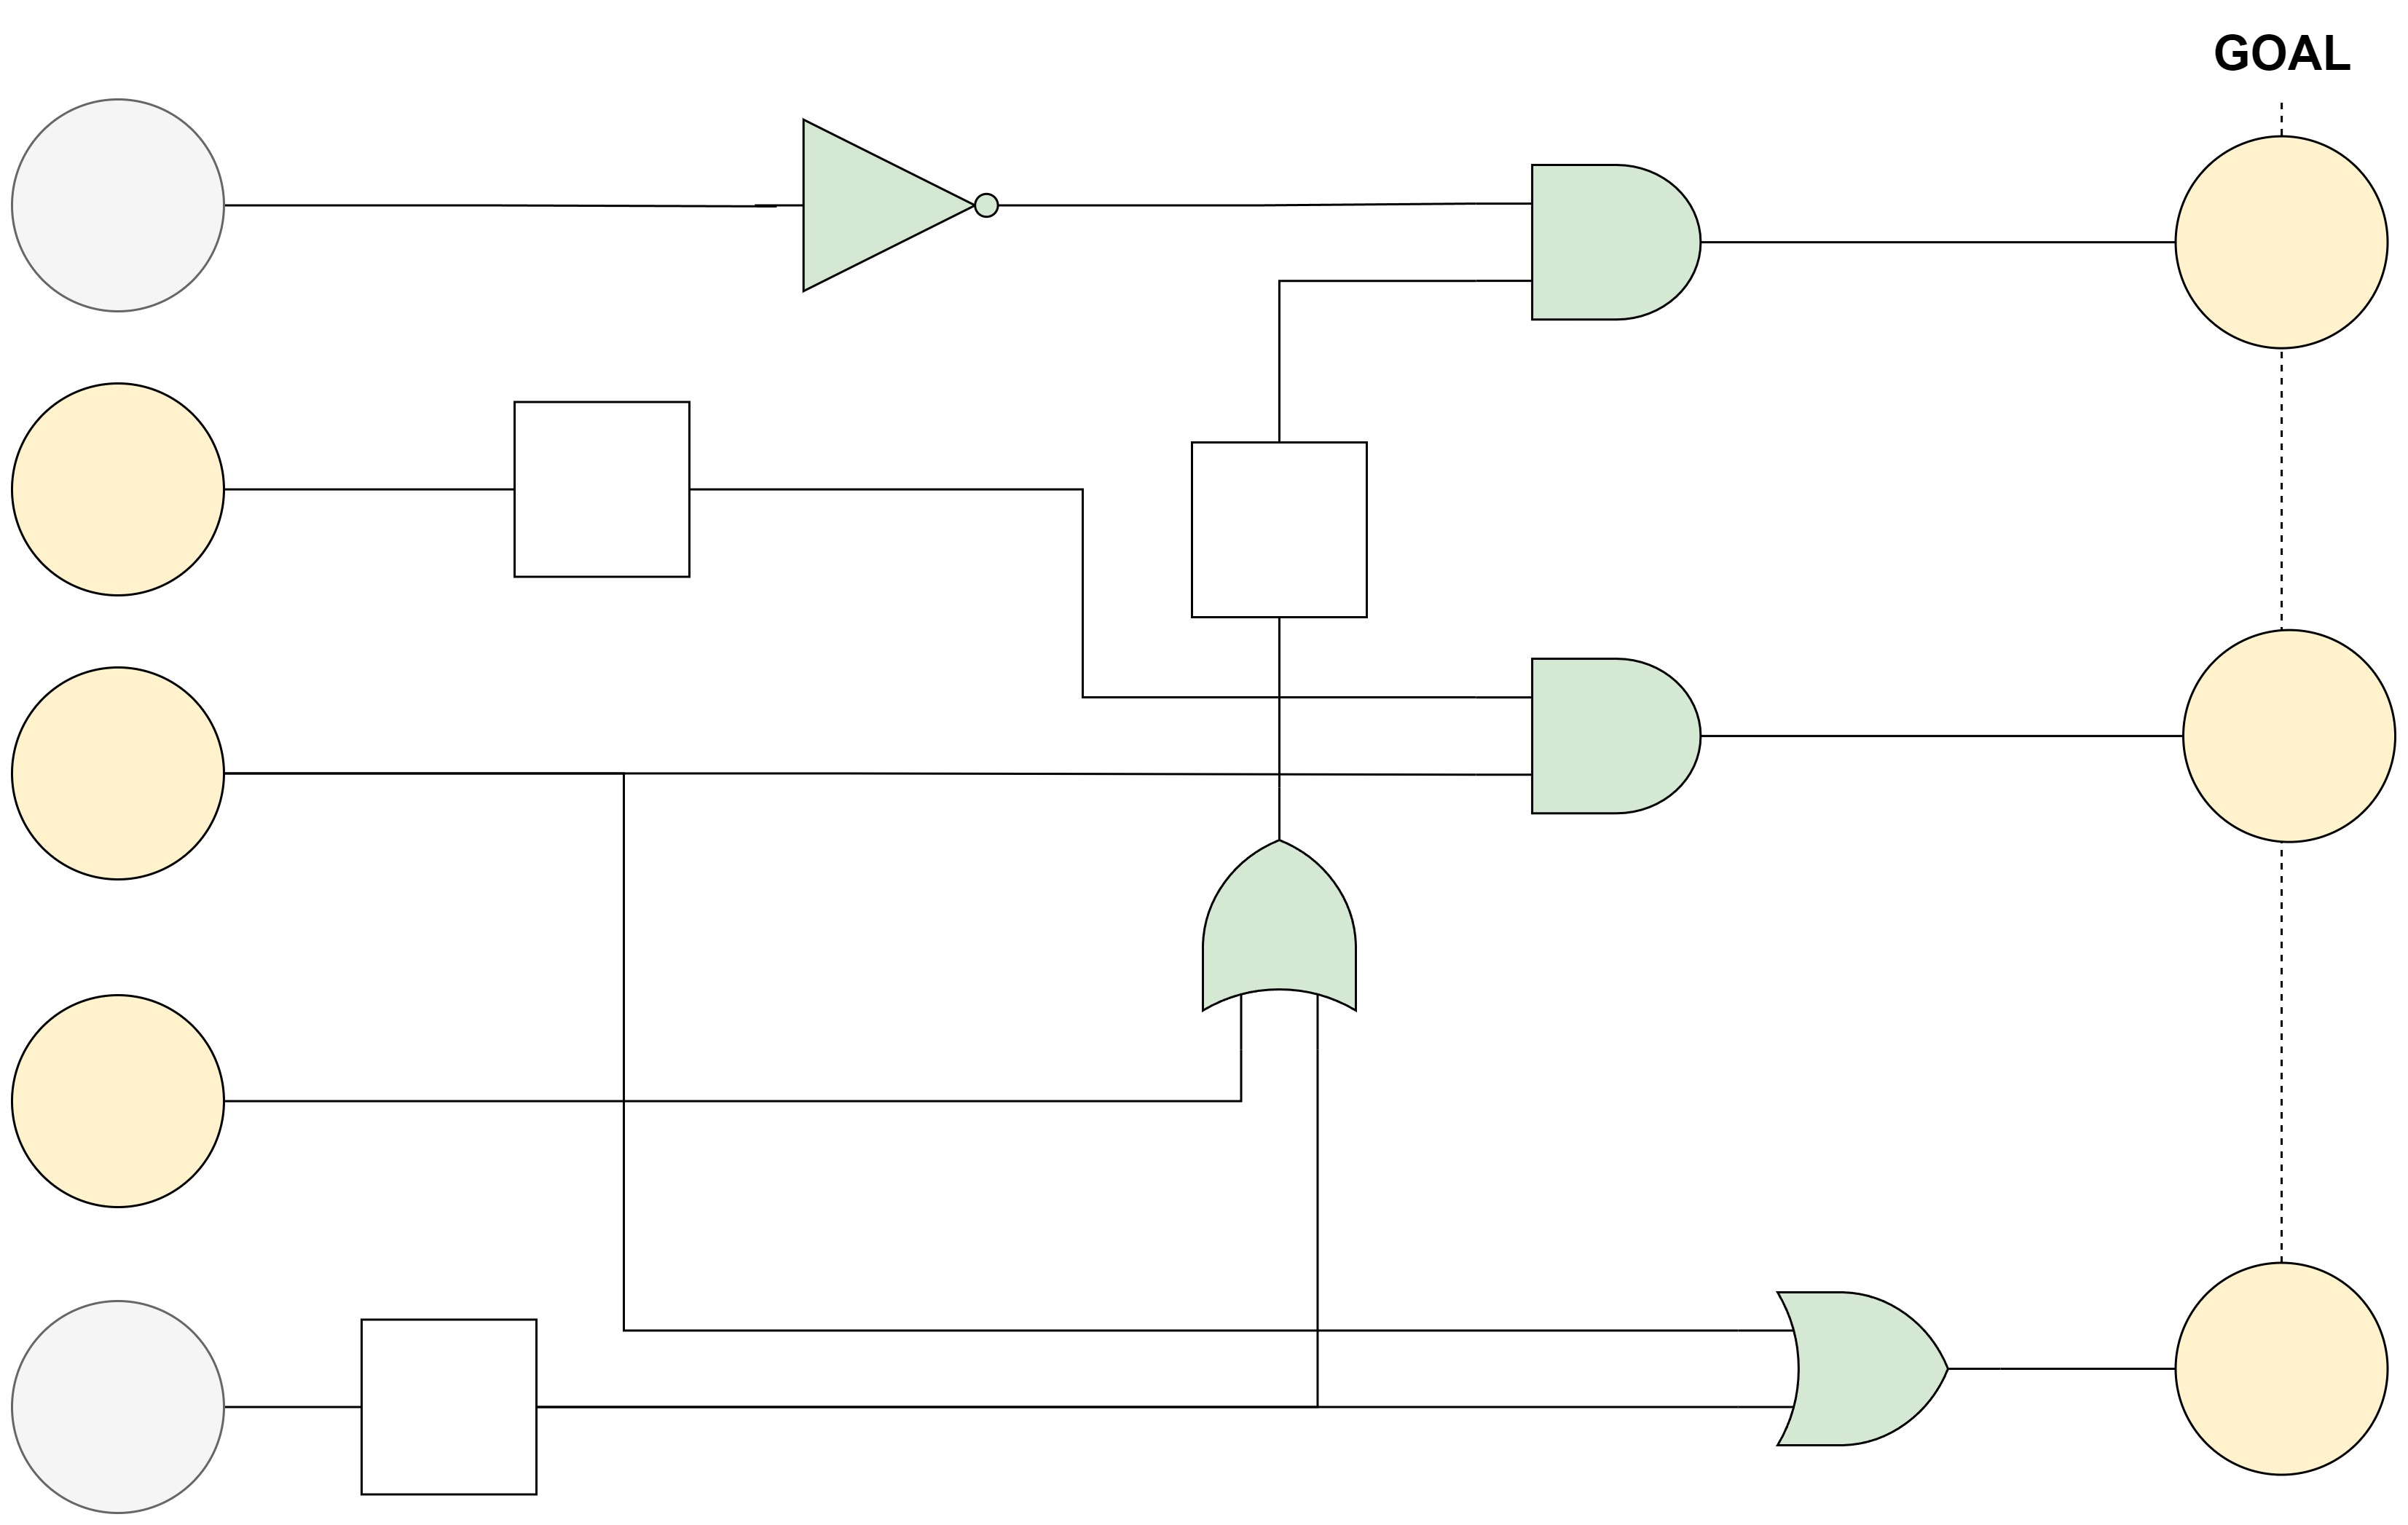
\includegraphics[width=\textwidth]{img/Levels-OR-3.jpg}
    \caption{3ème Niveau de la porte OR}
\end{figure}

\begin{figure}[h]
    \centering
    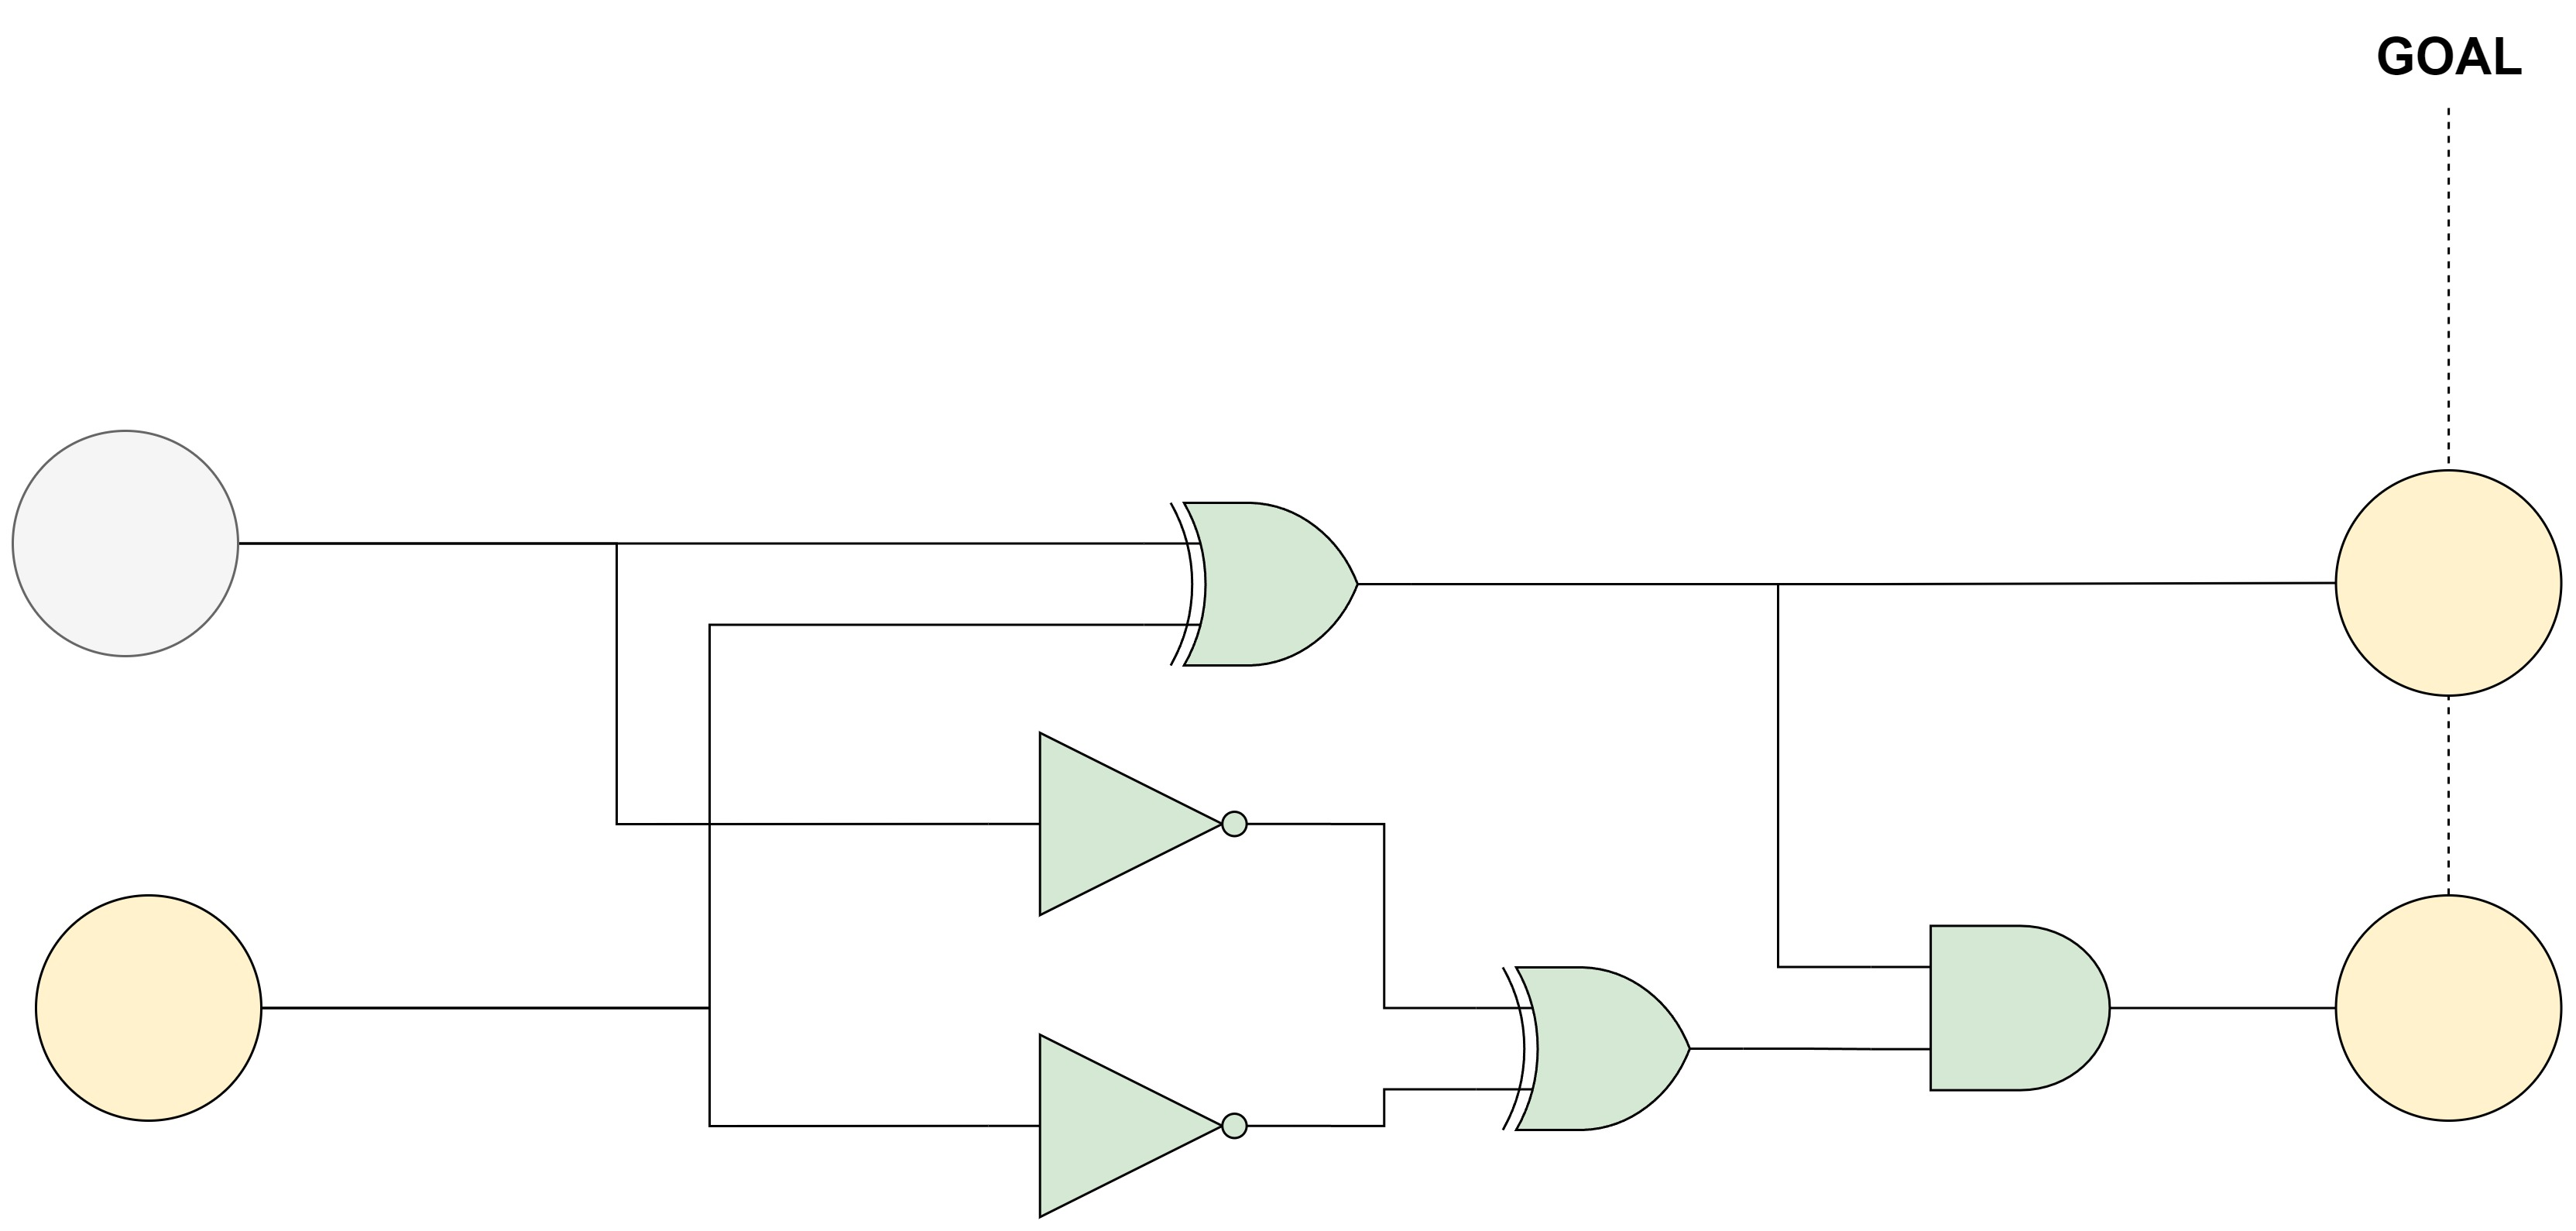
\includegraphics[width=\textwidth]{img/Levels-XOR-1.jpg}
    \caption{Premier Niveau de la porte XOR}
\end{figure}
\begin{figure}[h]
    \centering
    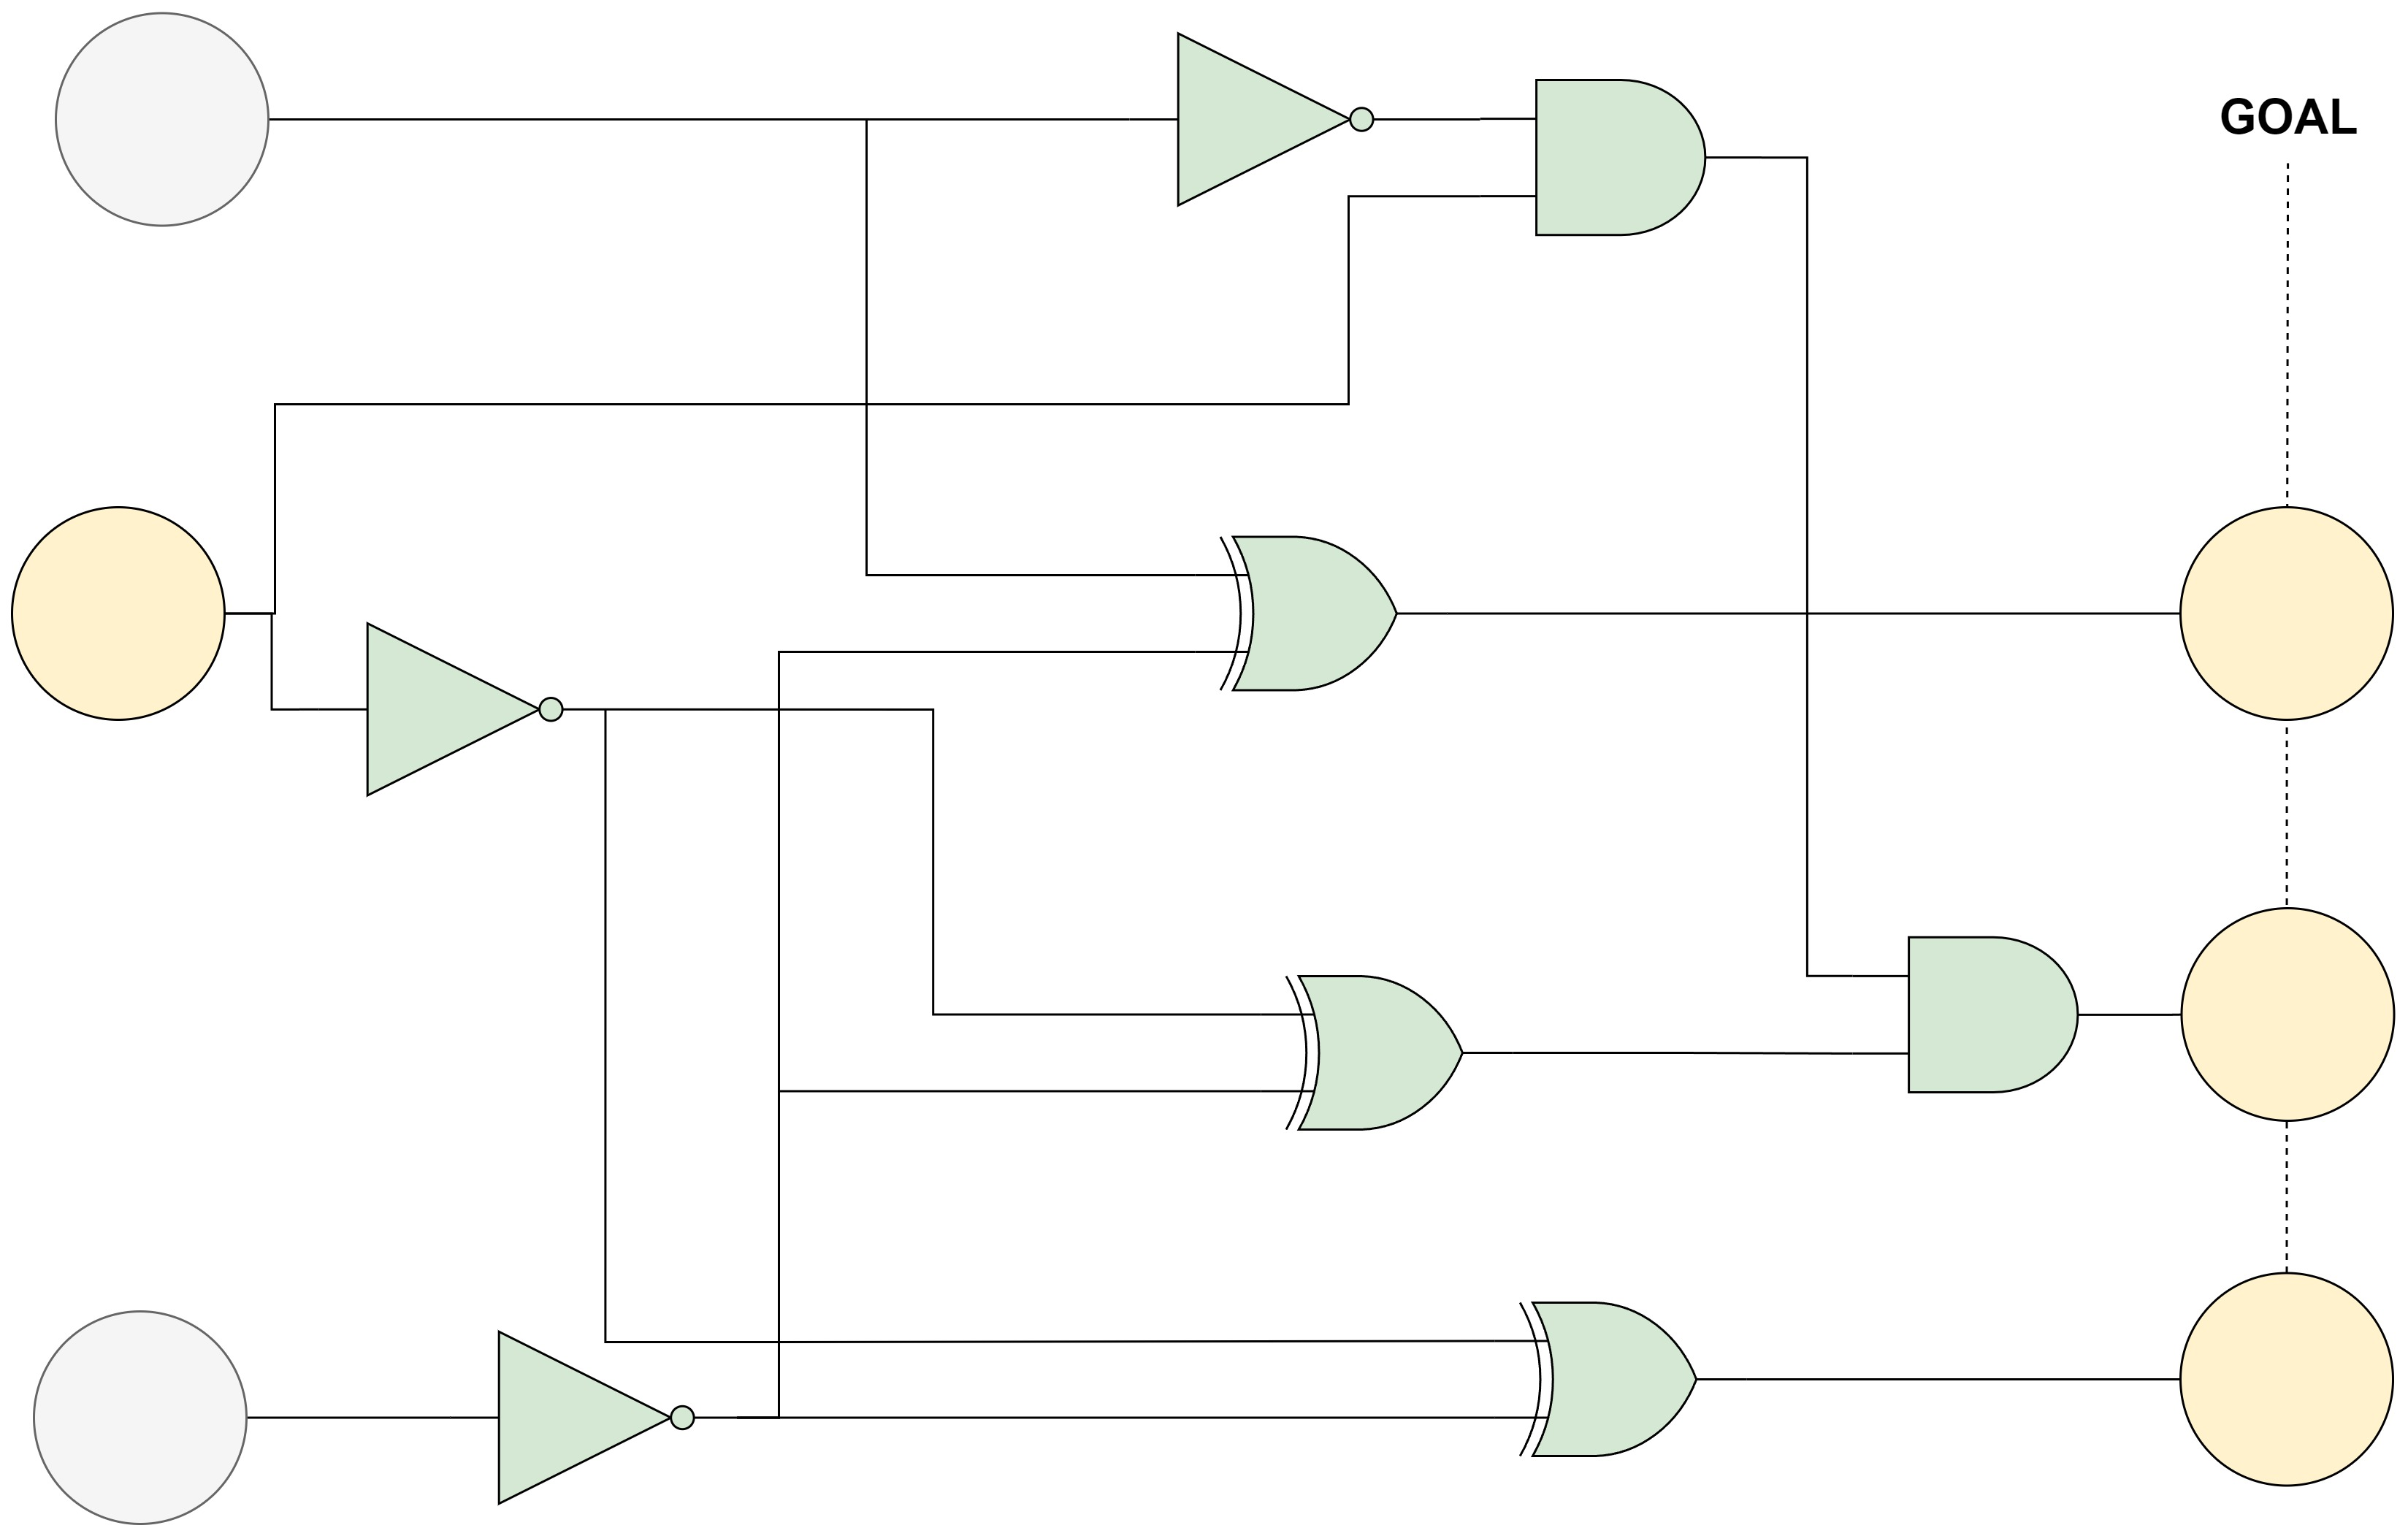
\includegraphics[width=\textwidth]{img/Levels-XOR-2.jpg}
    \caption{2ème Niveau de la porte XOR}
\end{figure}

\begin{figure}[h]
    \centering
    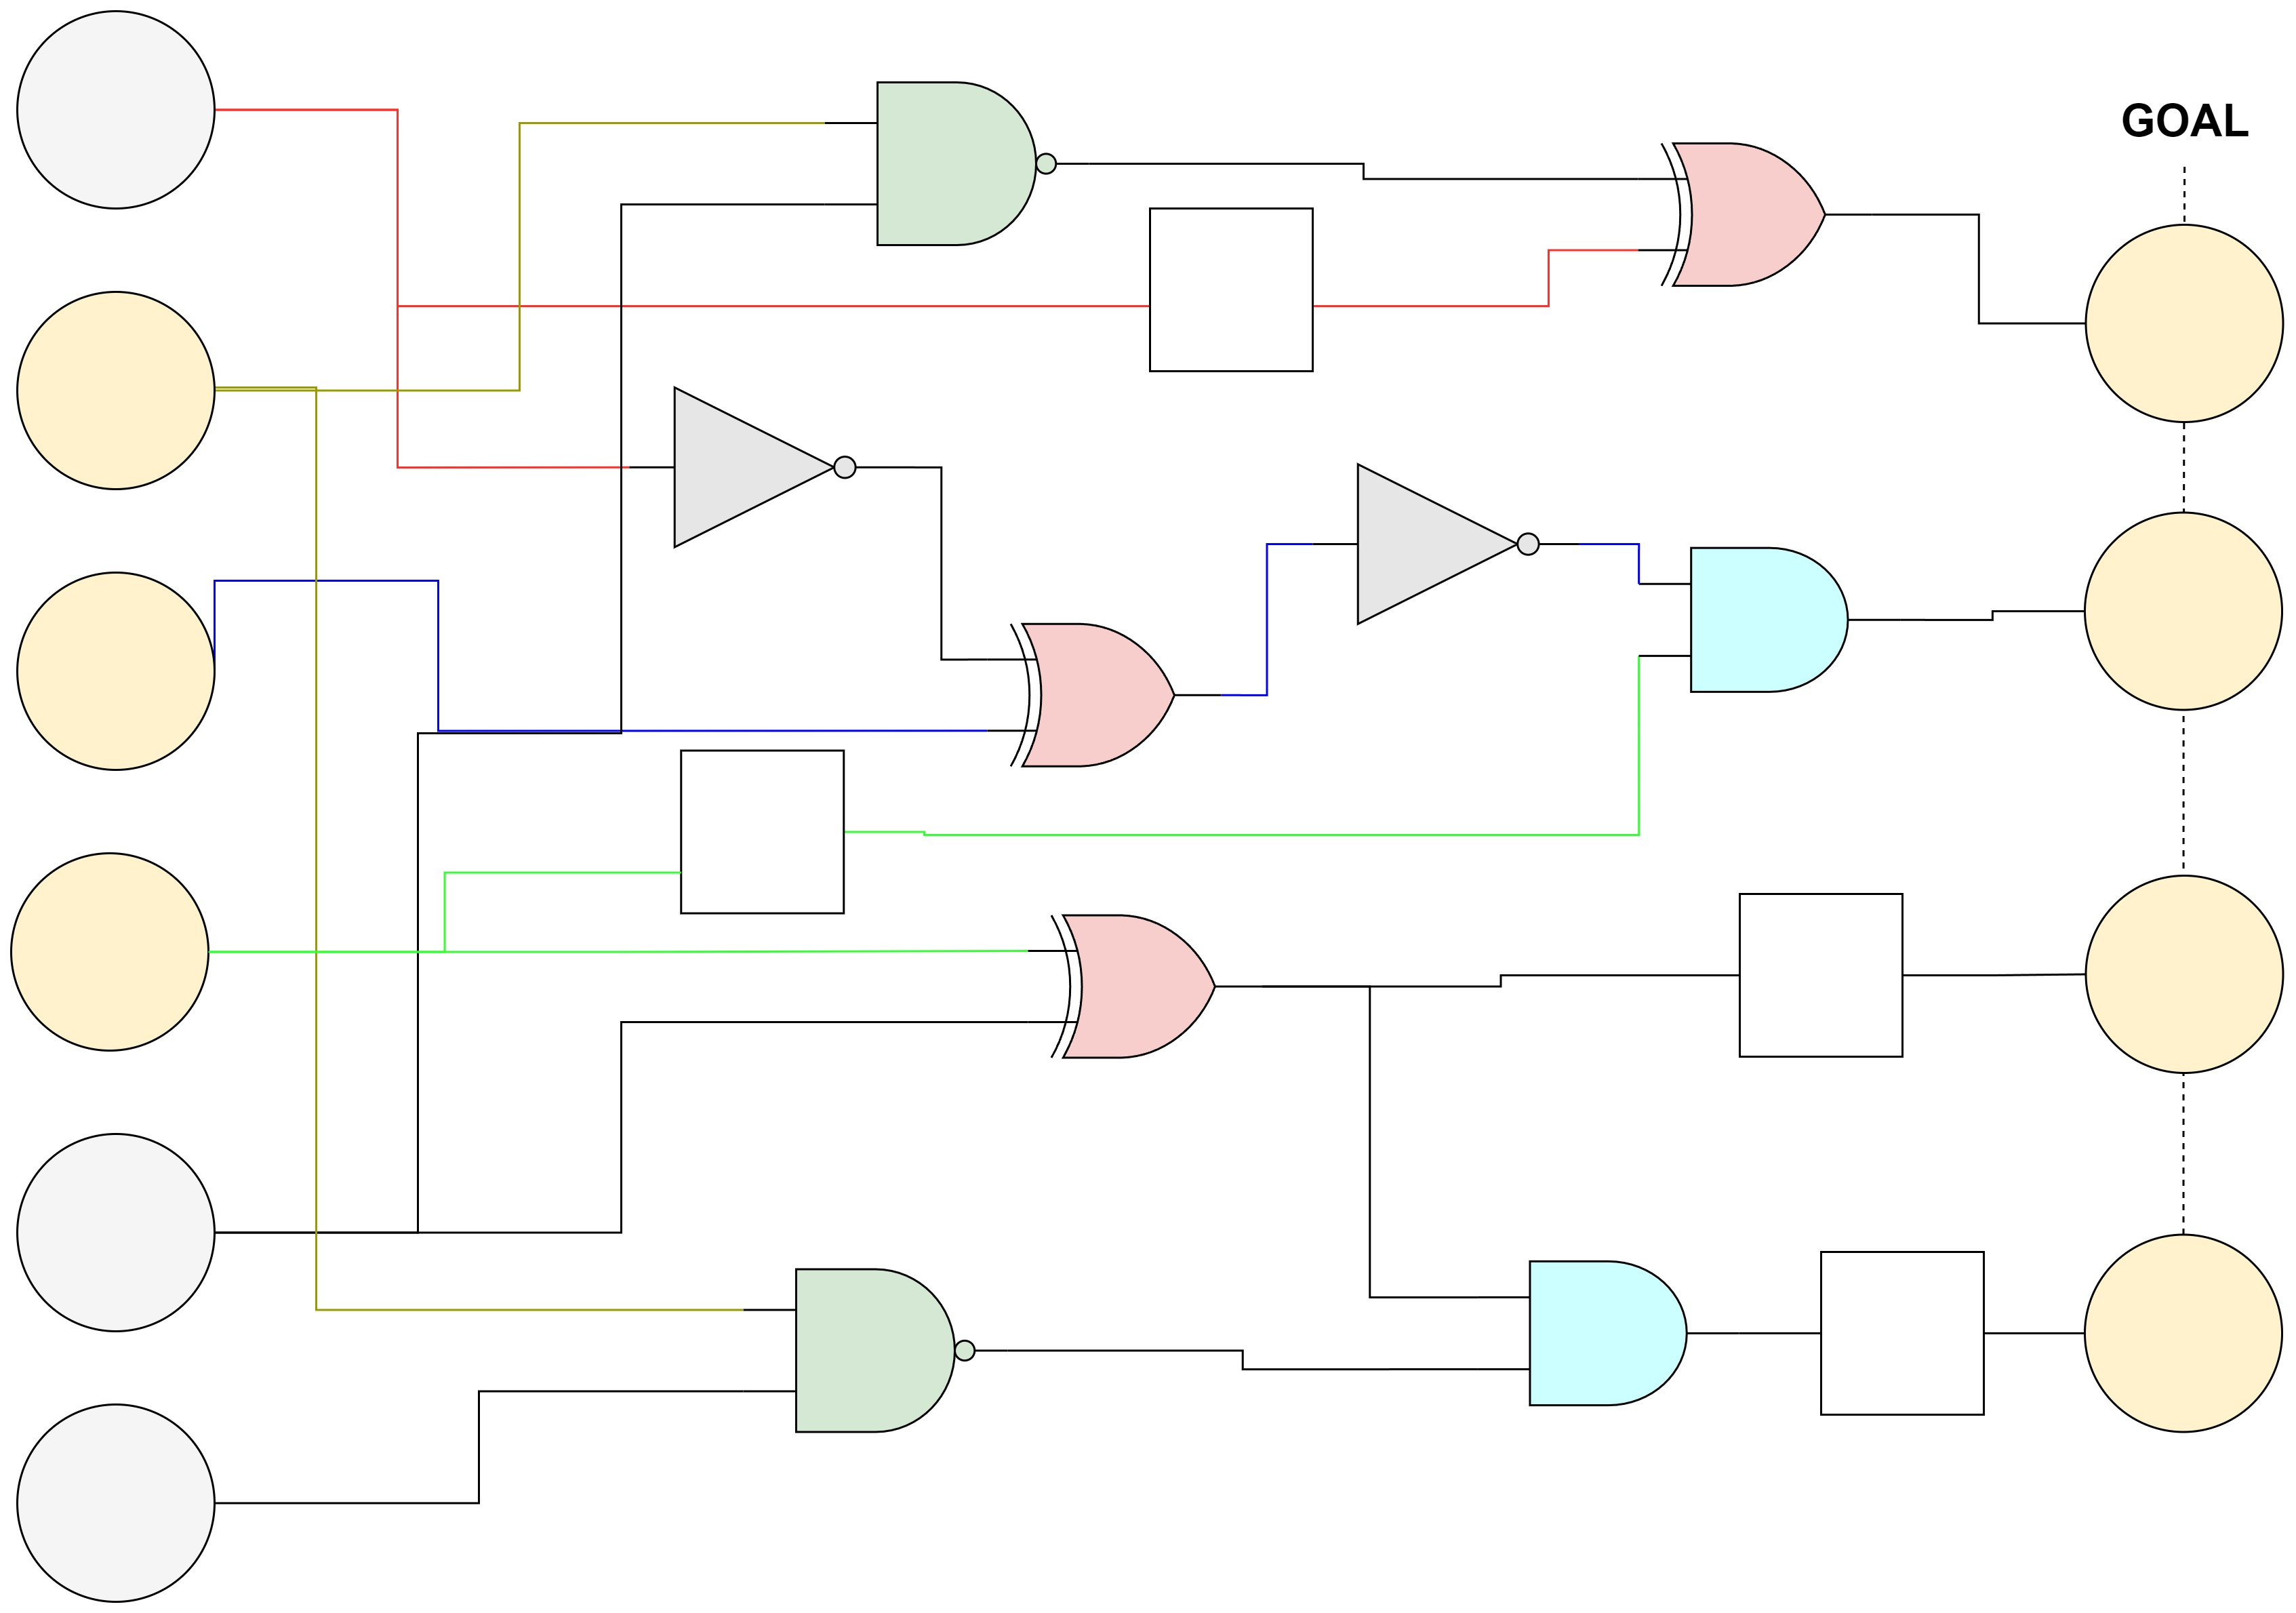
\includegraphics[width=\textwidth]{img/Levels-NAND-2.jpg}
    \caption{Niveau de la porte NAND (Niveau Final pour le cas où le joueur a réussi tous les niveaux précédents dans le temps impartit)}
\end{figure}

\end{document}
\[\]